\documentclass{article}
\usepackage[normalem]{ulem}
\usepackage[utf8]{inputenc}
\usepackage{graphicx}
\usepackage{mathtools}
\usepackage{amssymb}
\usepackage{amsmath}
\usepackage{macros}
\usepackage{color}

\begin{document}
\section{1. Plan area}

Repetition
% img 1
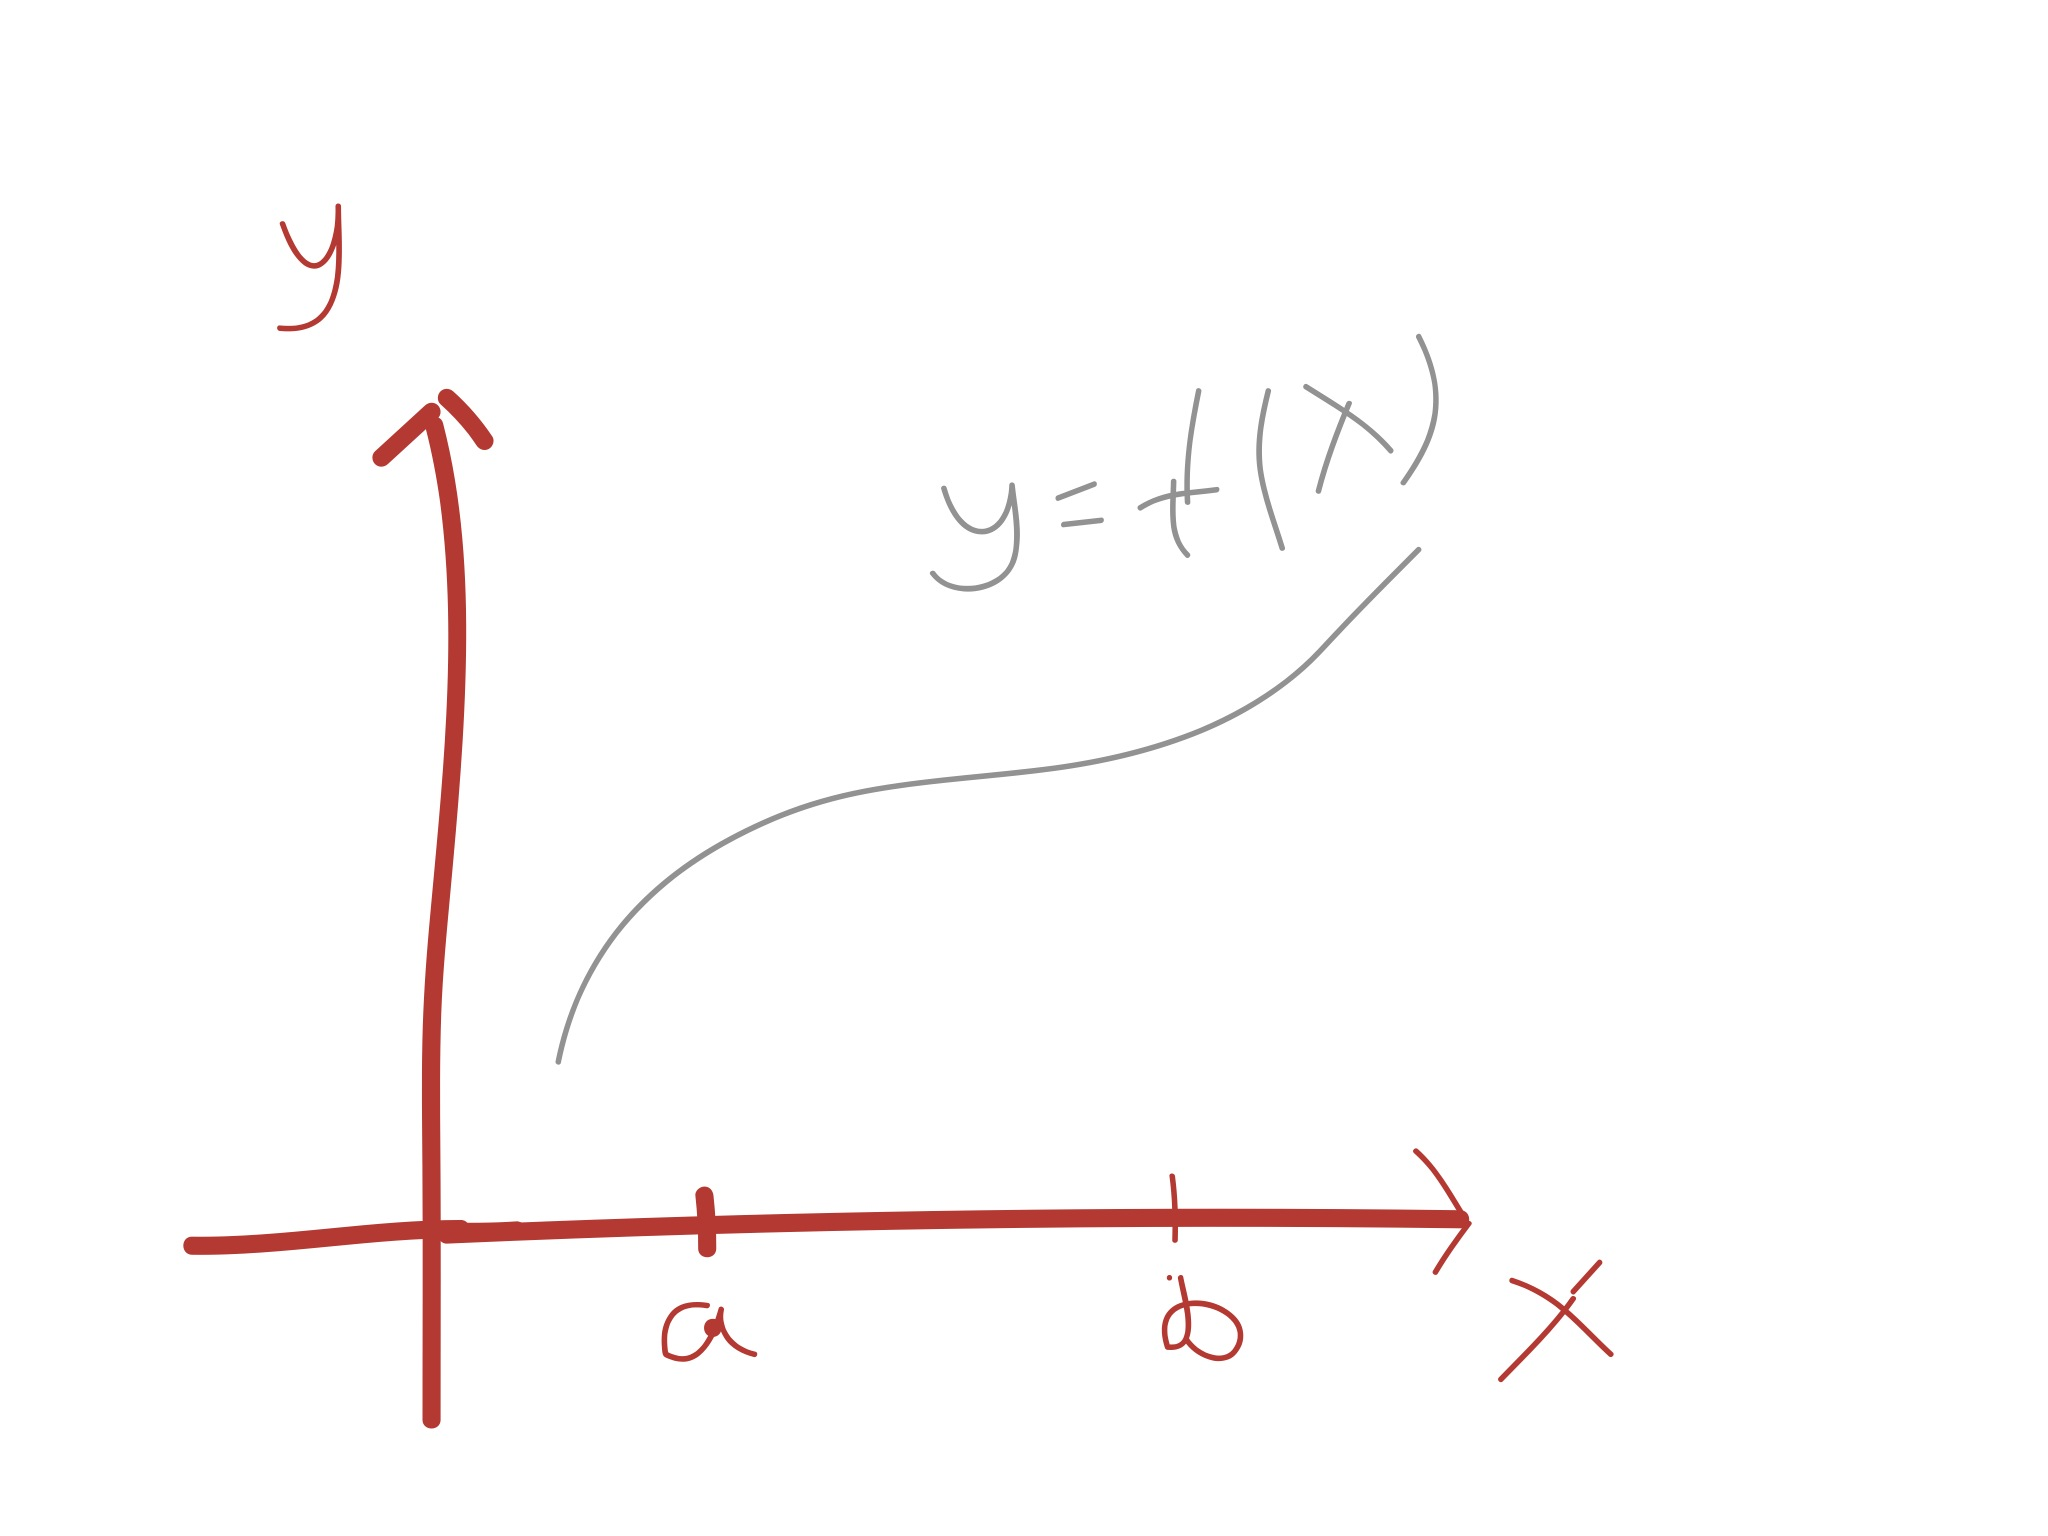
\includegraphics[scale=0.15]{img/img1.jpg}

$$ \int_a^b{f(x)\ dx} =\lim \sum_k{f(x_k) \Delta x_k}  $$

$$ D=\{(x,y) : a \le x \le b, g(x) \le y \le f(x)\} $$ där g, f är kontinuerliga.

% img 2
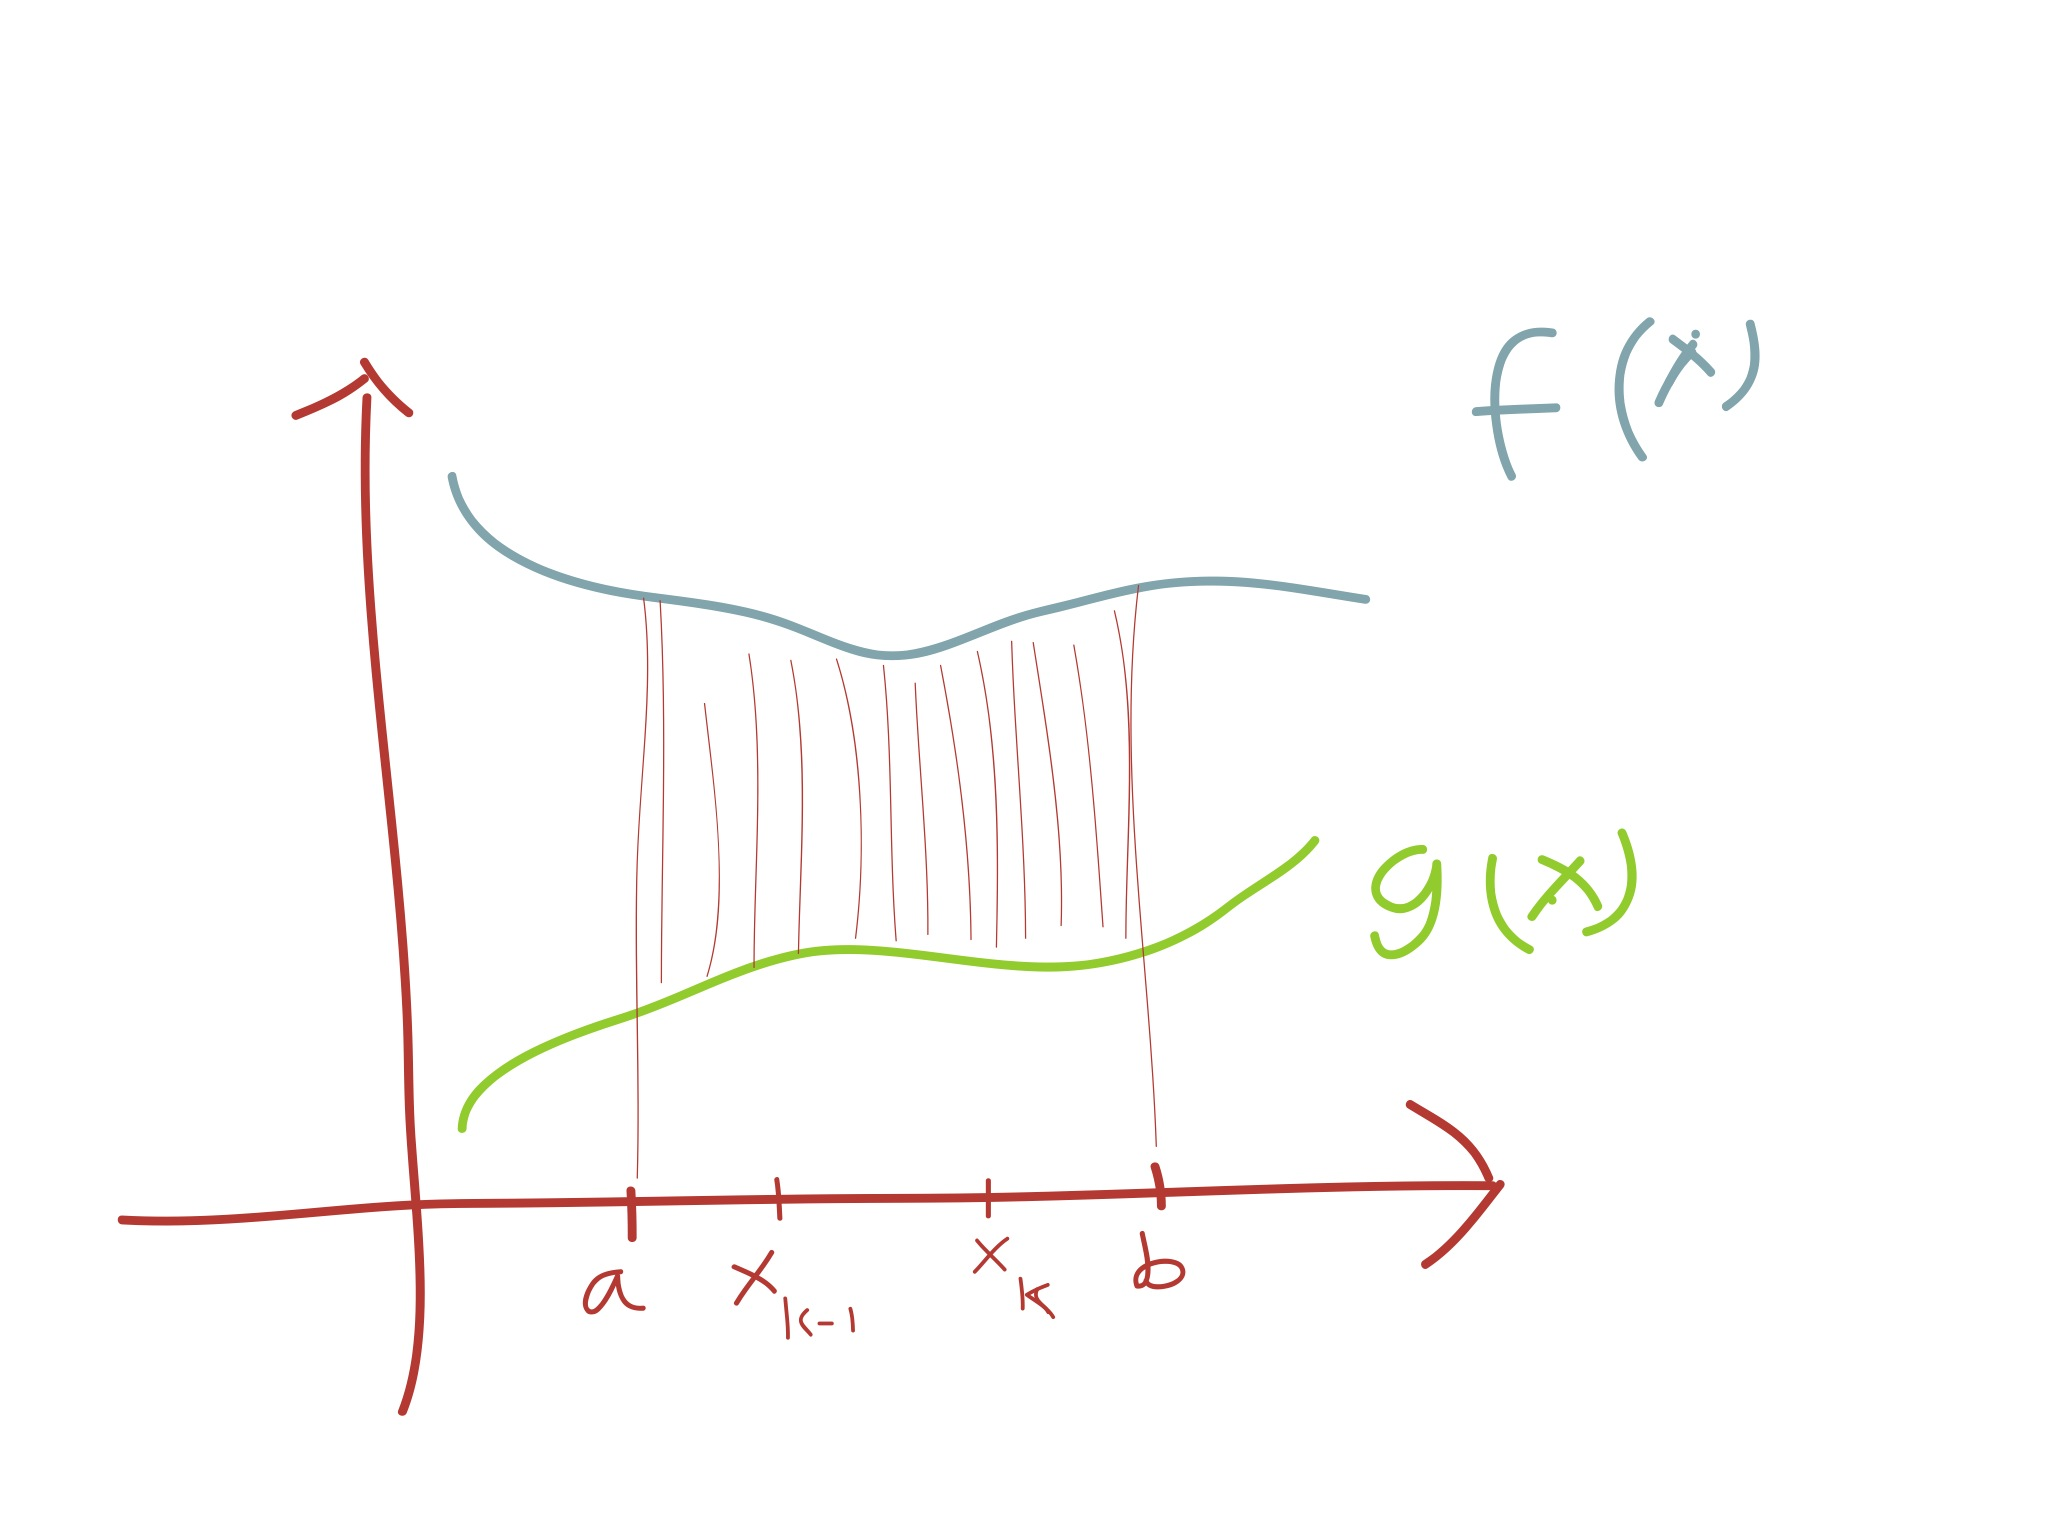
\includegraphics[scale=0.15]{img/img2.jpg}

$$ A(D) = \int_a^b{(f(x) - g(x))\ dx} $$

% img 3
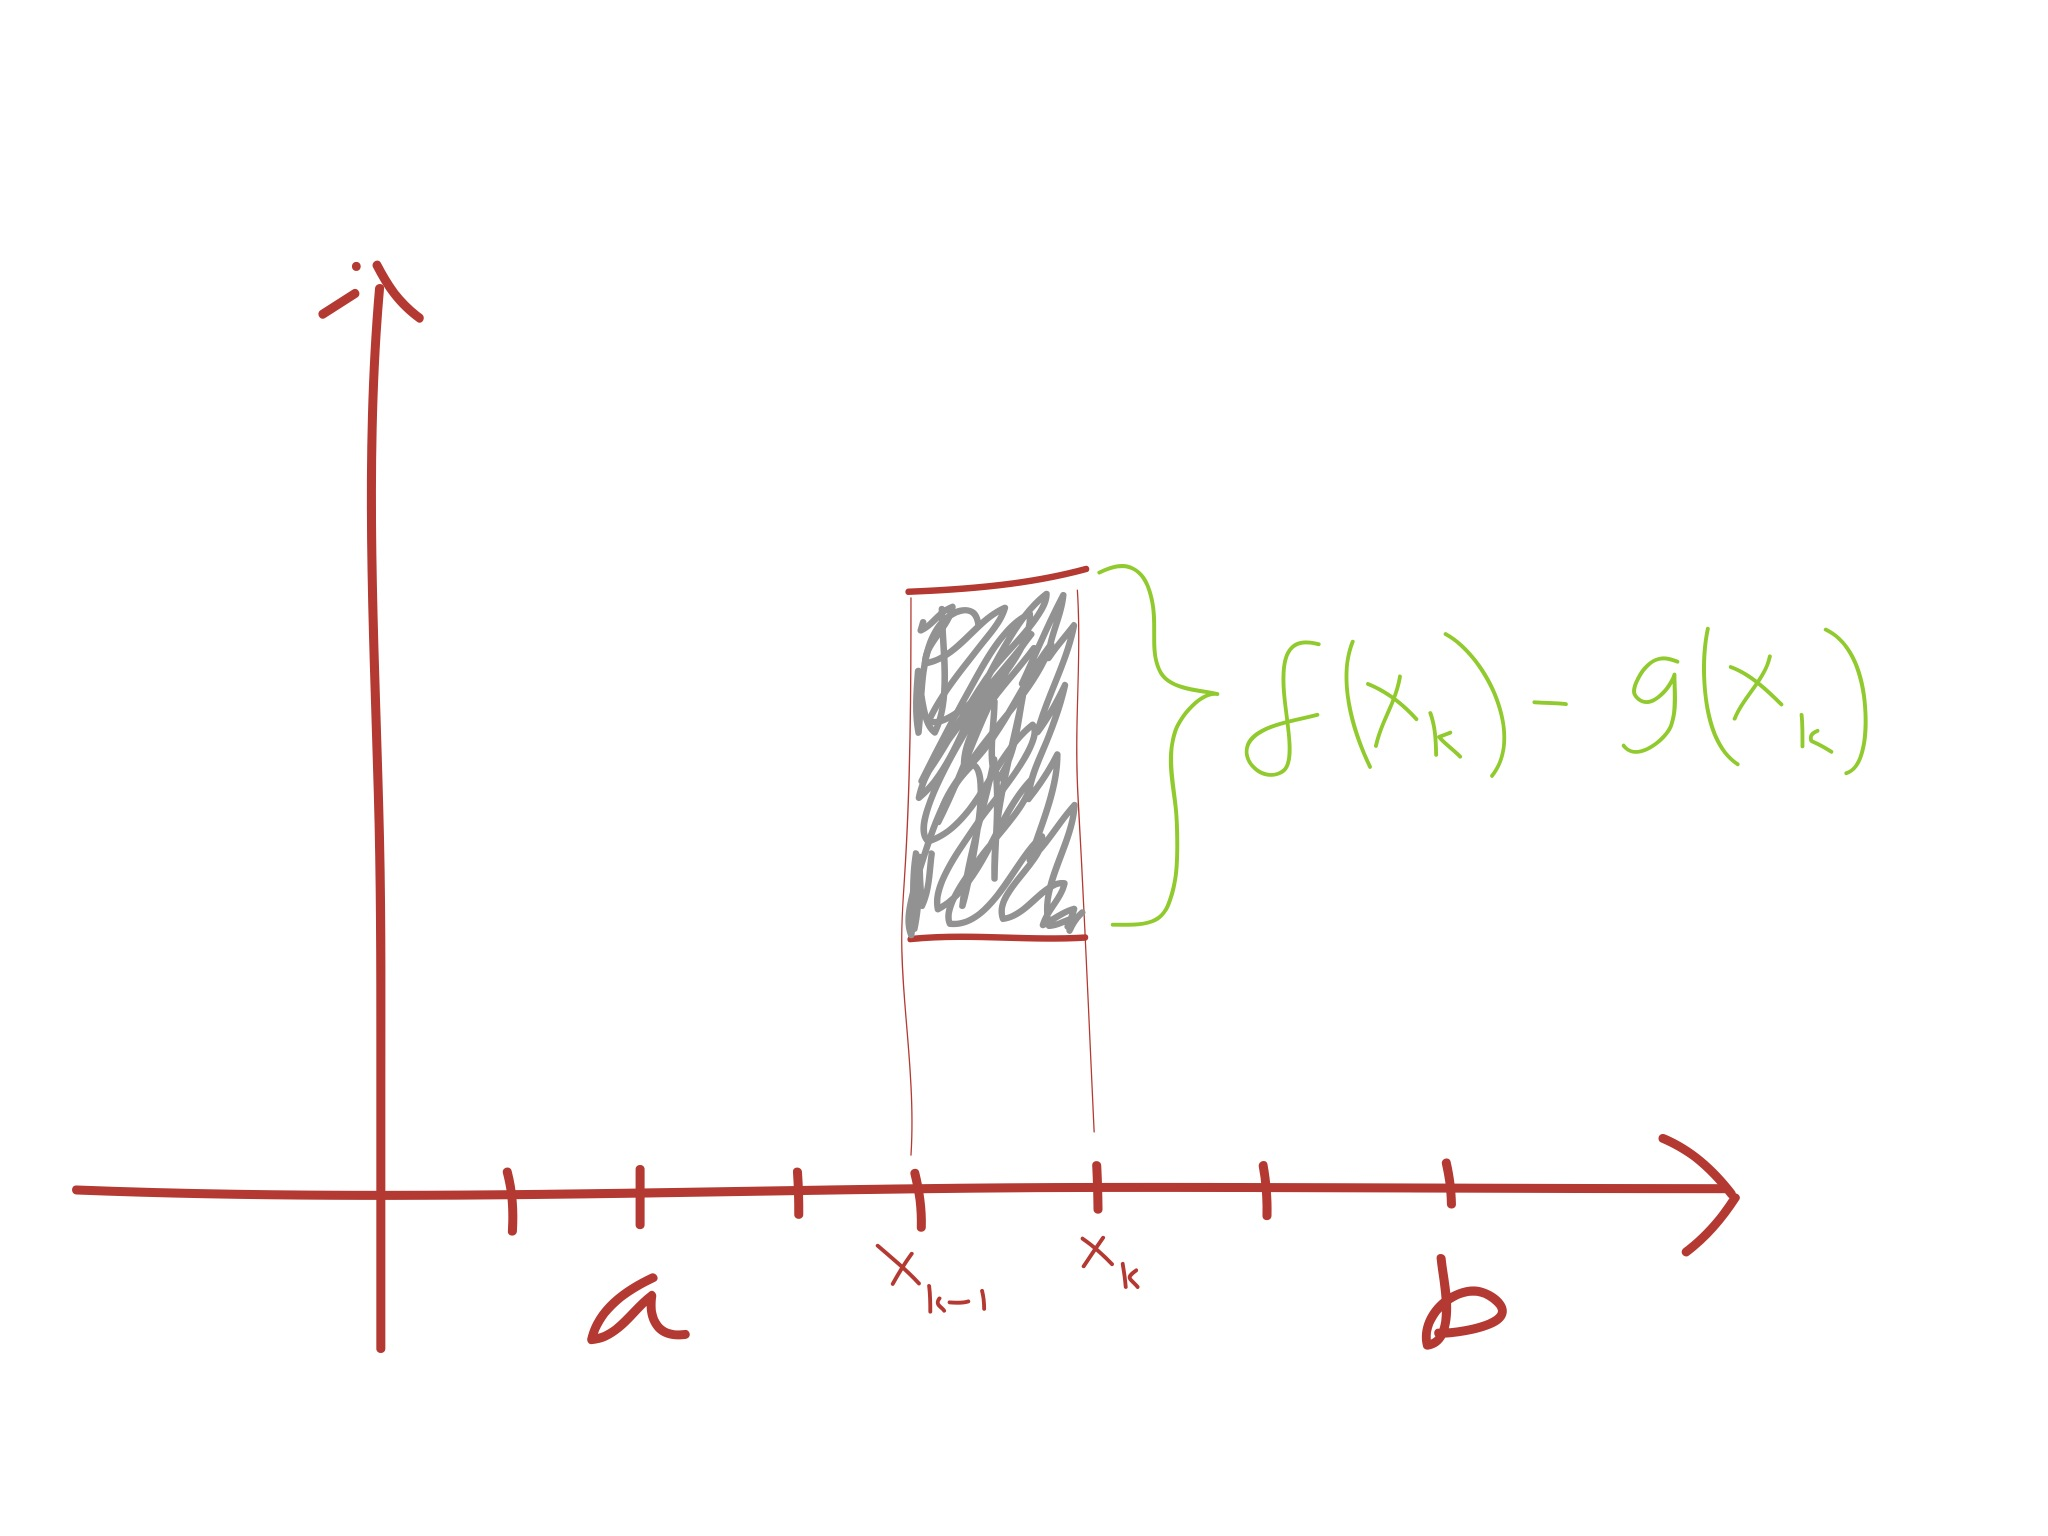
\includegraphics[scale=0.15]{img/img3.jpg}

$$ \Delta x_k = x_k - x_{k-1} $$

$$ \Delta A_k \approx (f(x_k)-g(x_k))\Delta x_k $$

$$ A(D) \approx \sum{\Delta A} = \sum{f(x_k) - g(x_k)} \Delta x_k $$

$$ \Delta x_k \to 0 \im A(D) = \int^b_a{(f(x) - g(x))\ dx} $$

\subsection{Exempel 1}
Bestäm arean av det område som begränsas av $y=x$ och $y=x^2$

% img 4
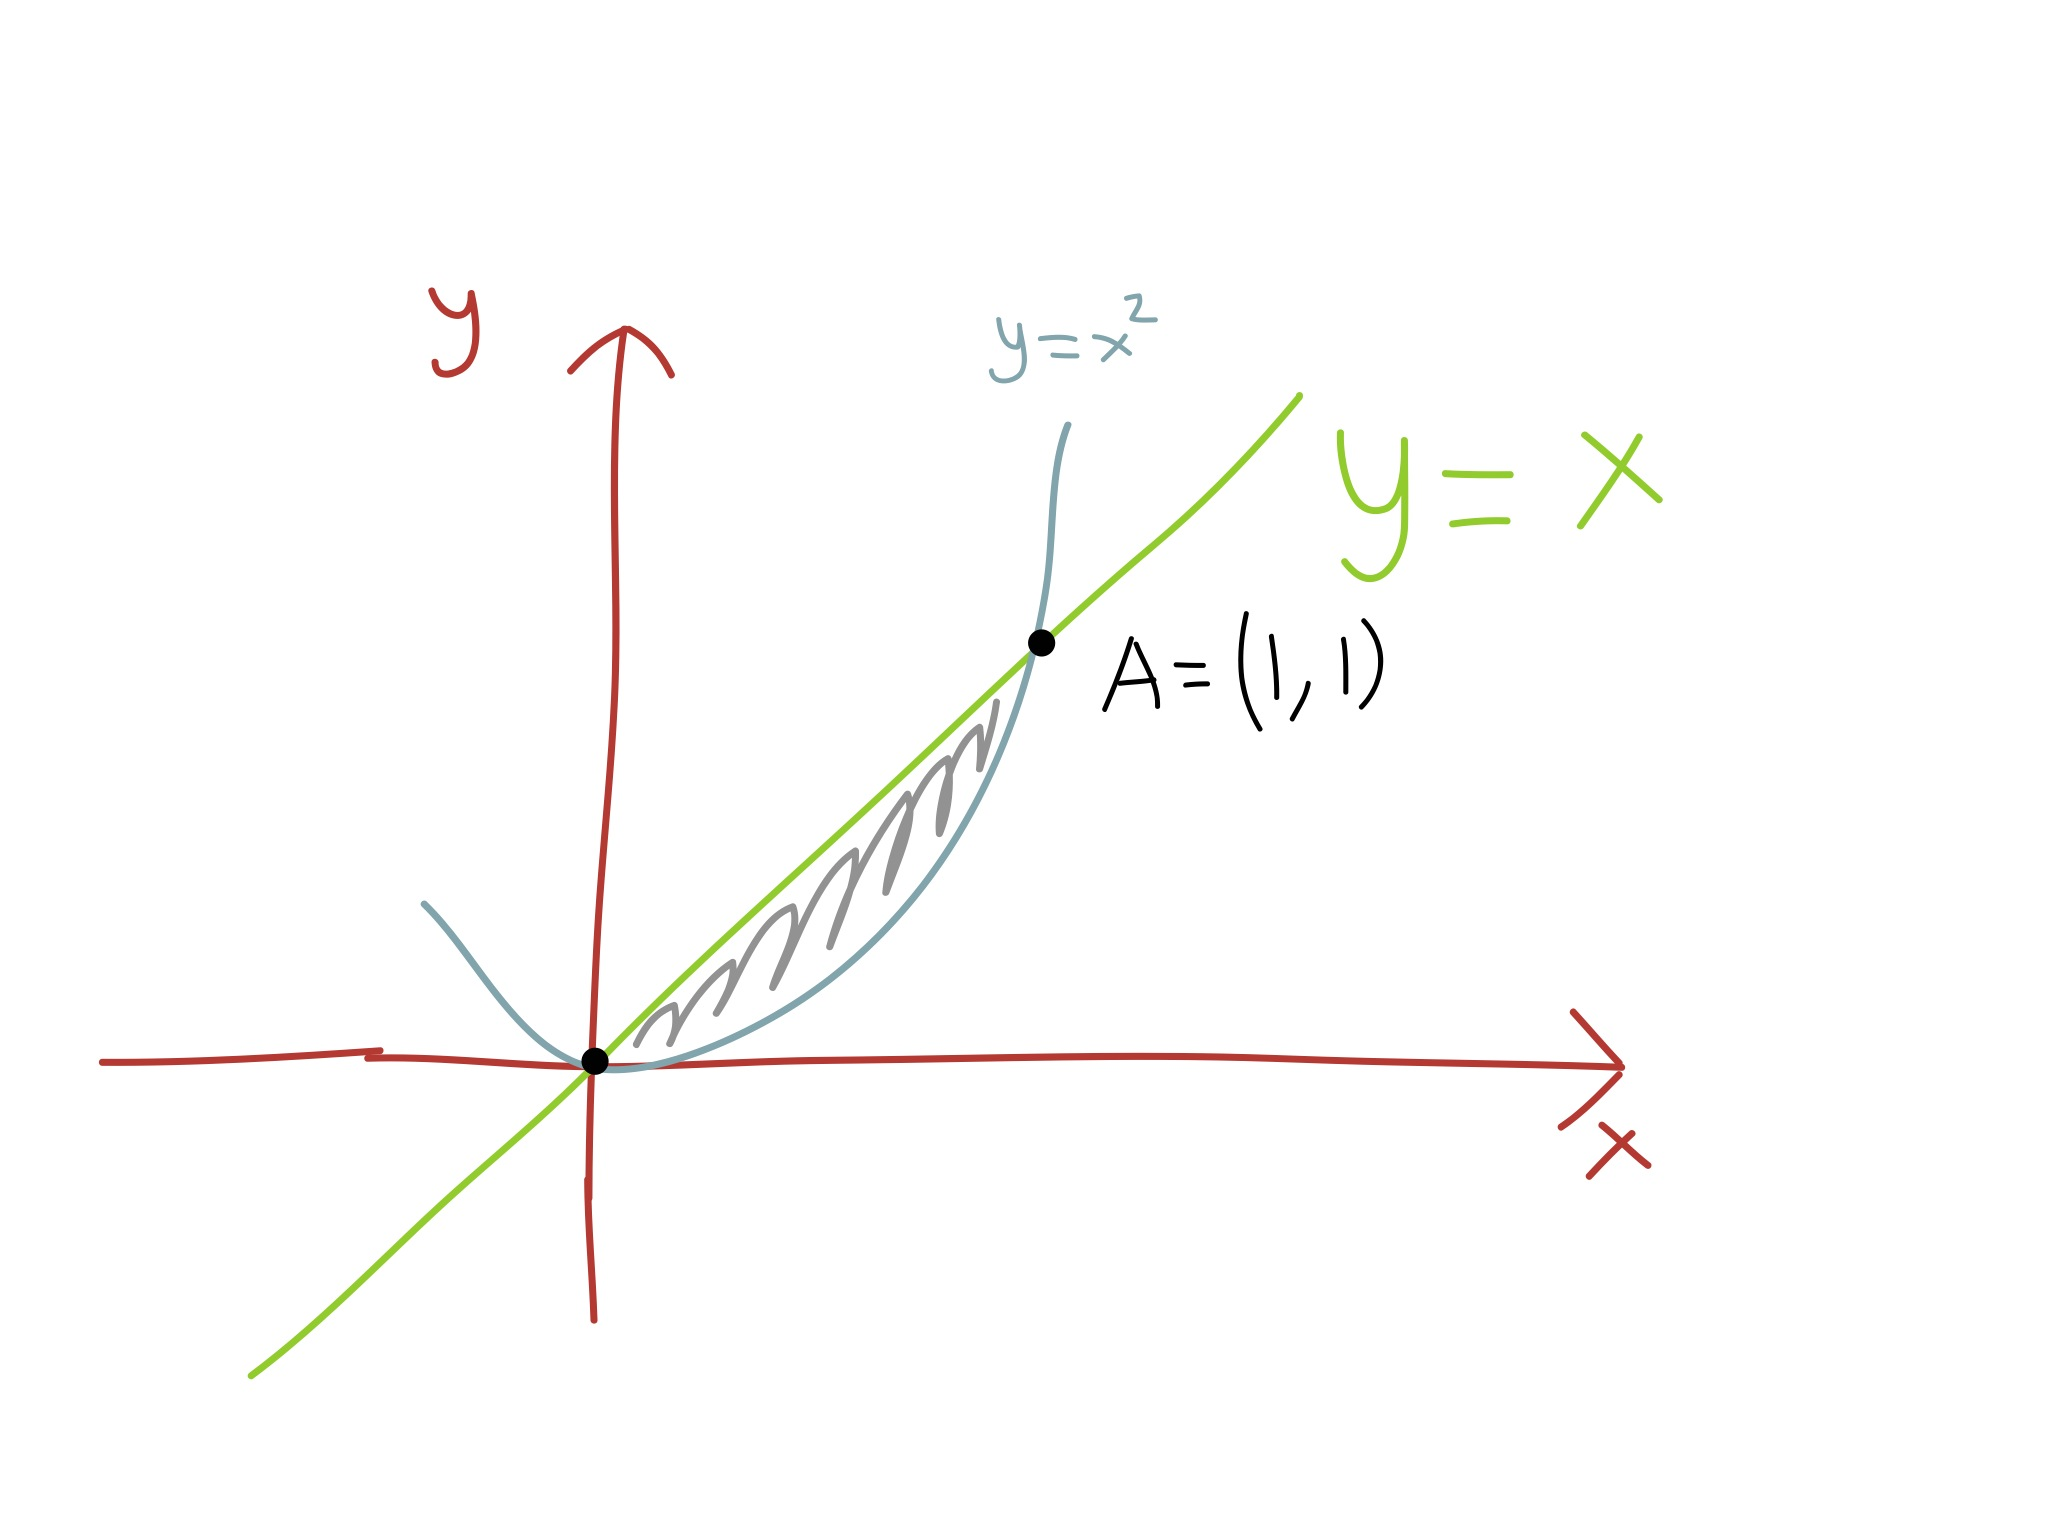
\includegraphics[scale=0.15]{img/img4.jpg}

$$ D=\{(x,y) : 0\le x \le 1, x^2 \le y\le x \} $$
$A(D) = \int^1_0{ (x-x^2)dx } = \bra{ \f{x^2}2 - \f{x^3}3 } = \f 16$

\section{Arean på polär form}
Polära koordinater $(\phi, r)$

% img 5
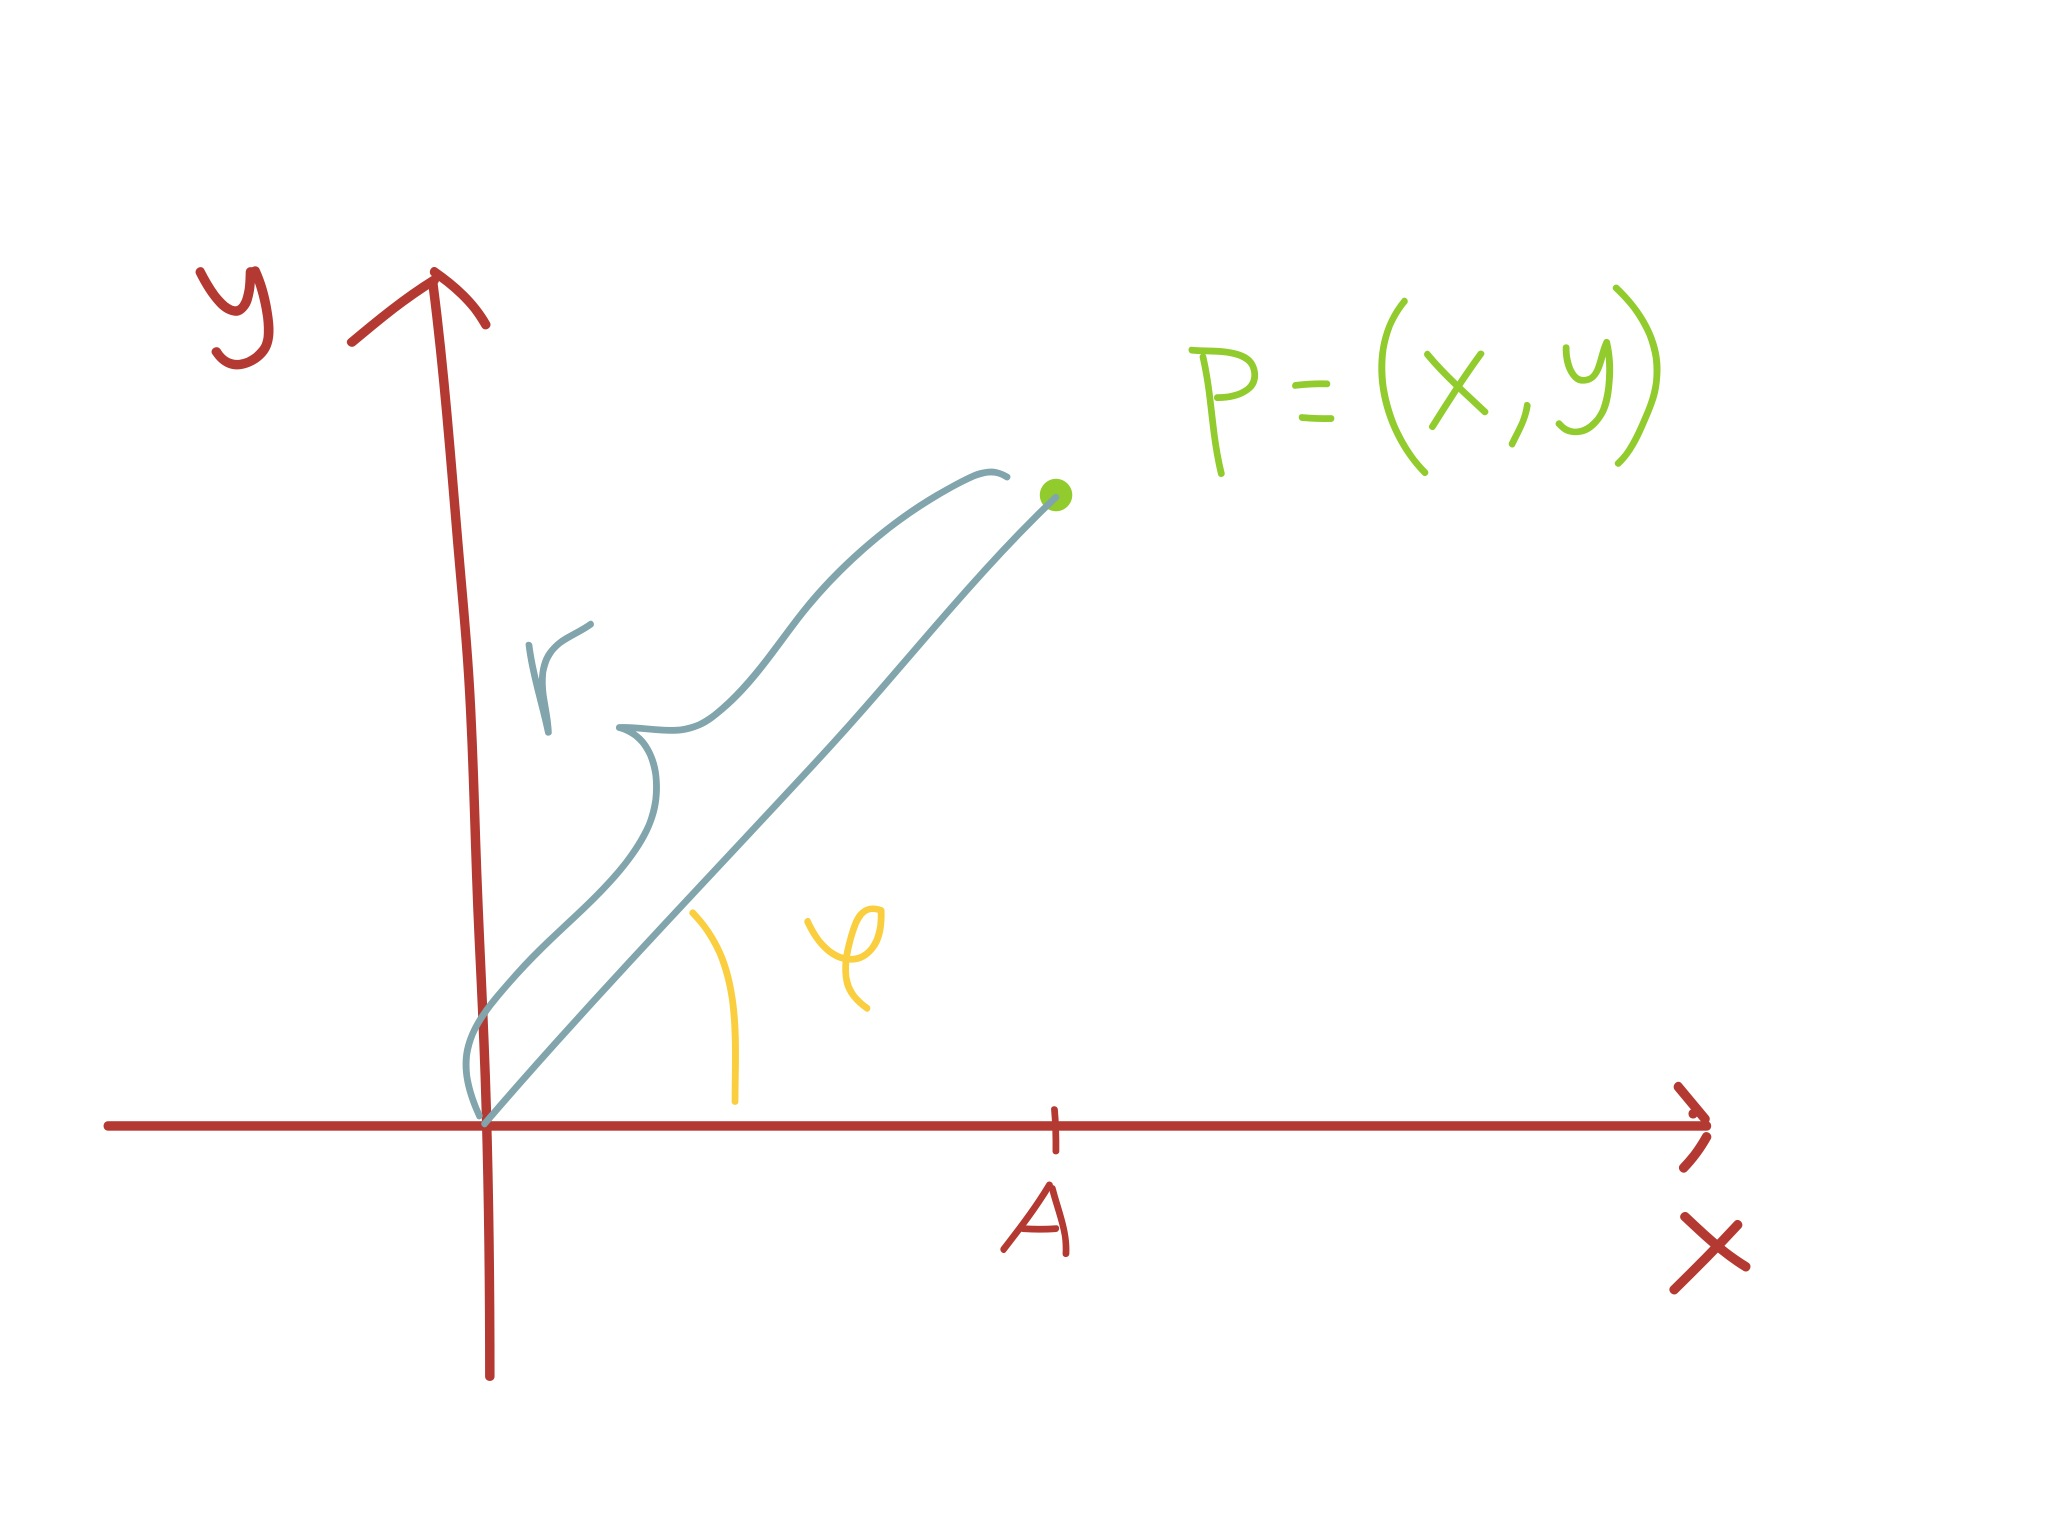
\includegraphics[scale=0.15]{img/img5.jpg}

$$
\begin{cases}
x=r\cos\phi\\
y=r\sin\phi
\end{cases}
$$

% img 6
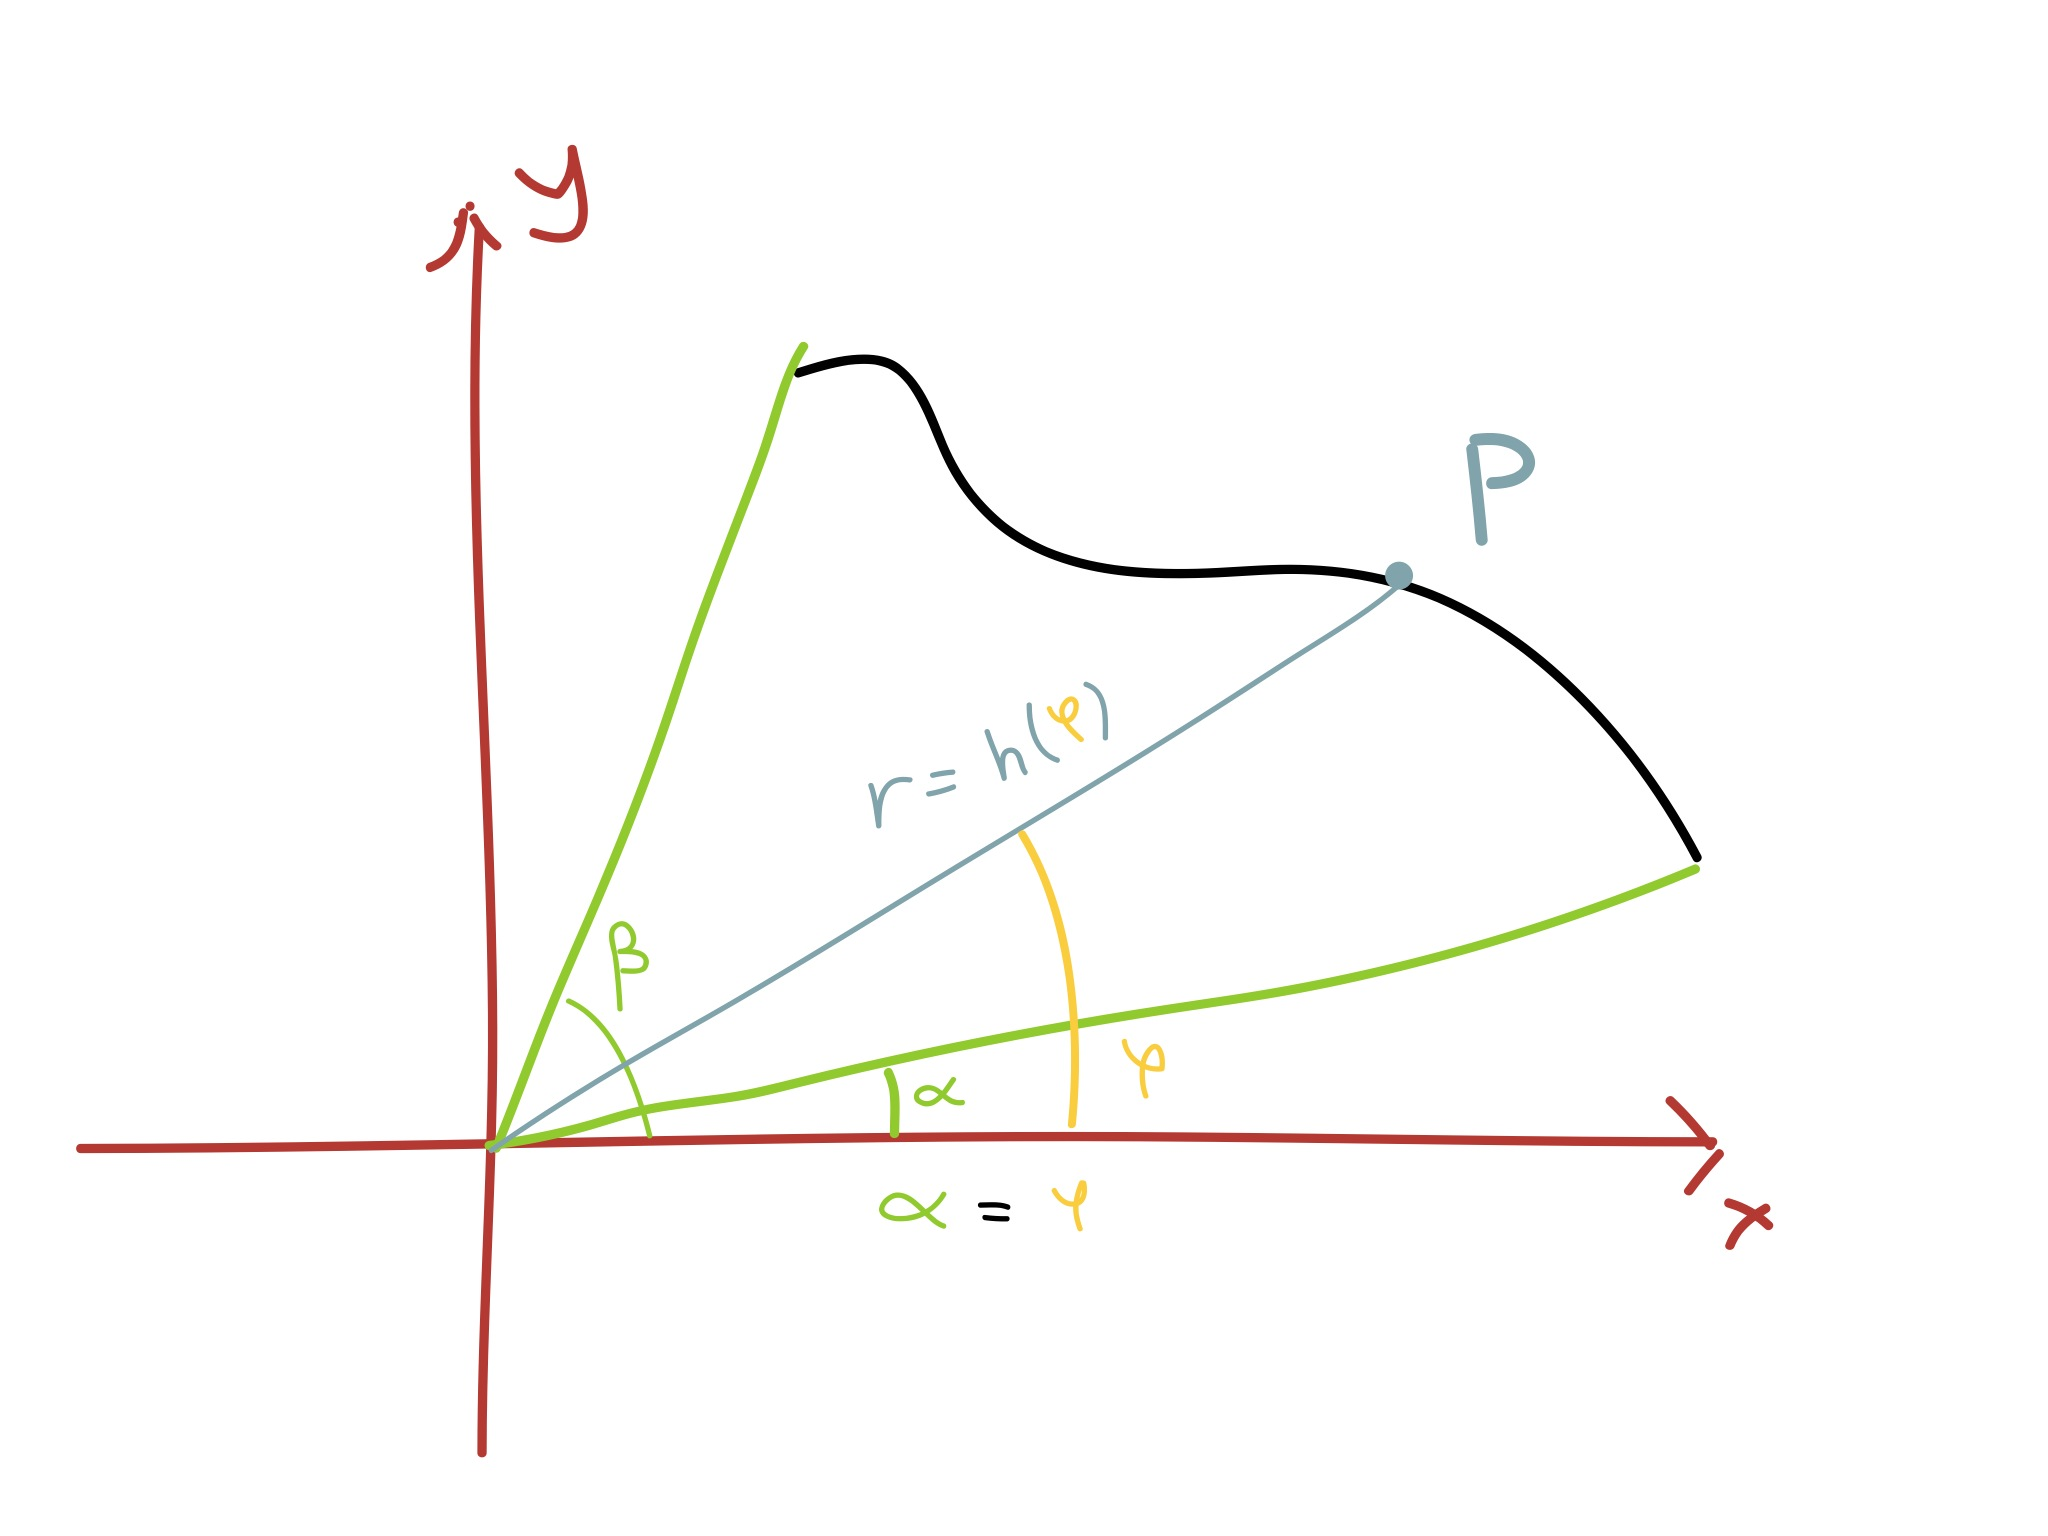
\includegraphics[scale=0.15]{img/img6.jpg}

$$ D = \{ (x, y) : \alpha\le\phi\le\beta, 0\le r\le h(\phi) $$

Om h är kontinuerlig då kan vi beräkna arean av D som:
$$ A(D) = \f 12 \int^\beta_\alpha{h^2(\phi)\ d\phi} $$

% img 7
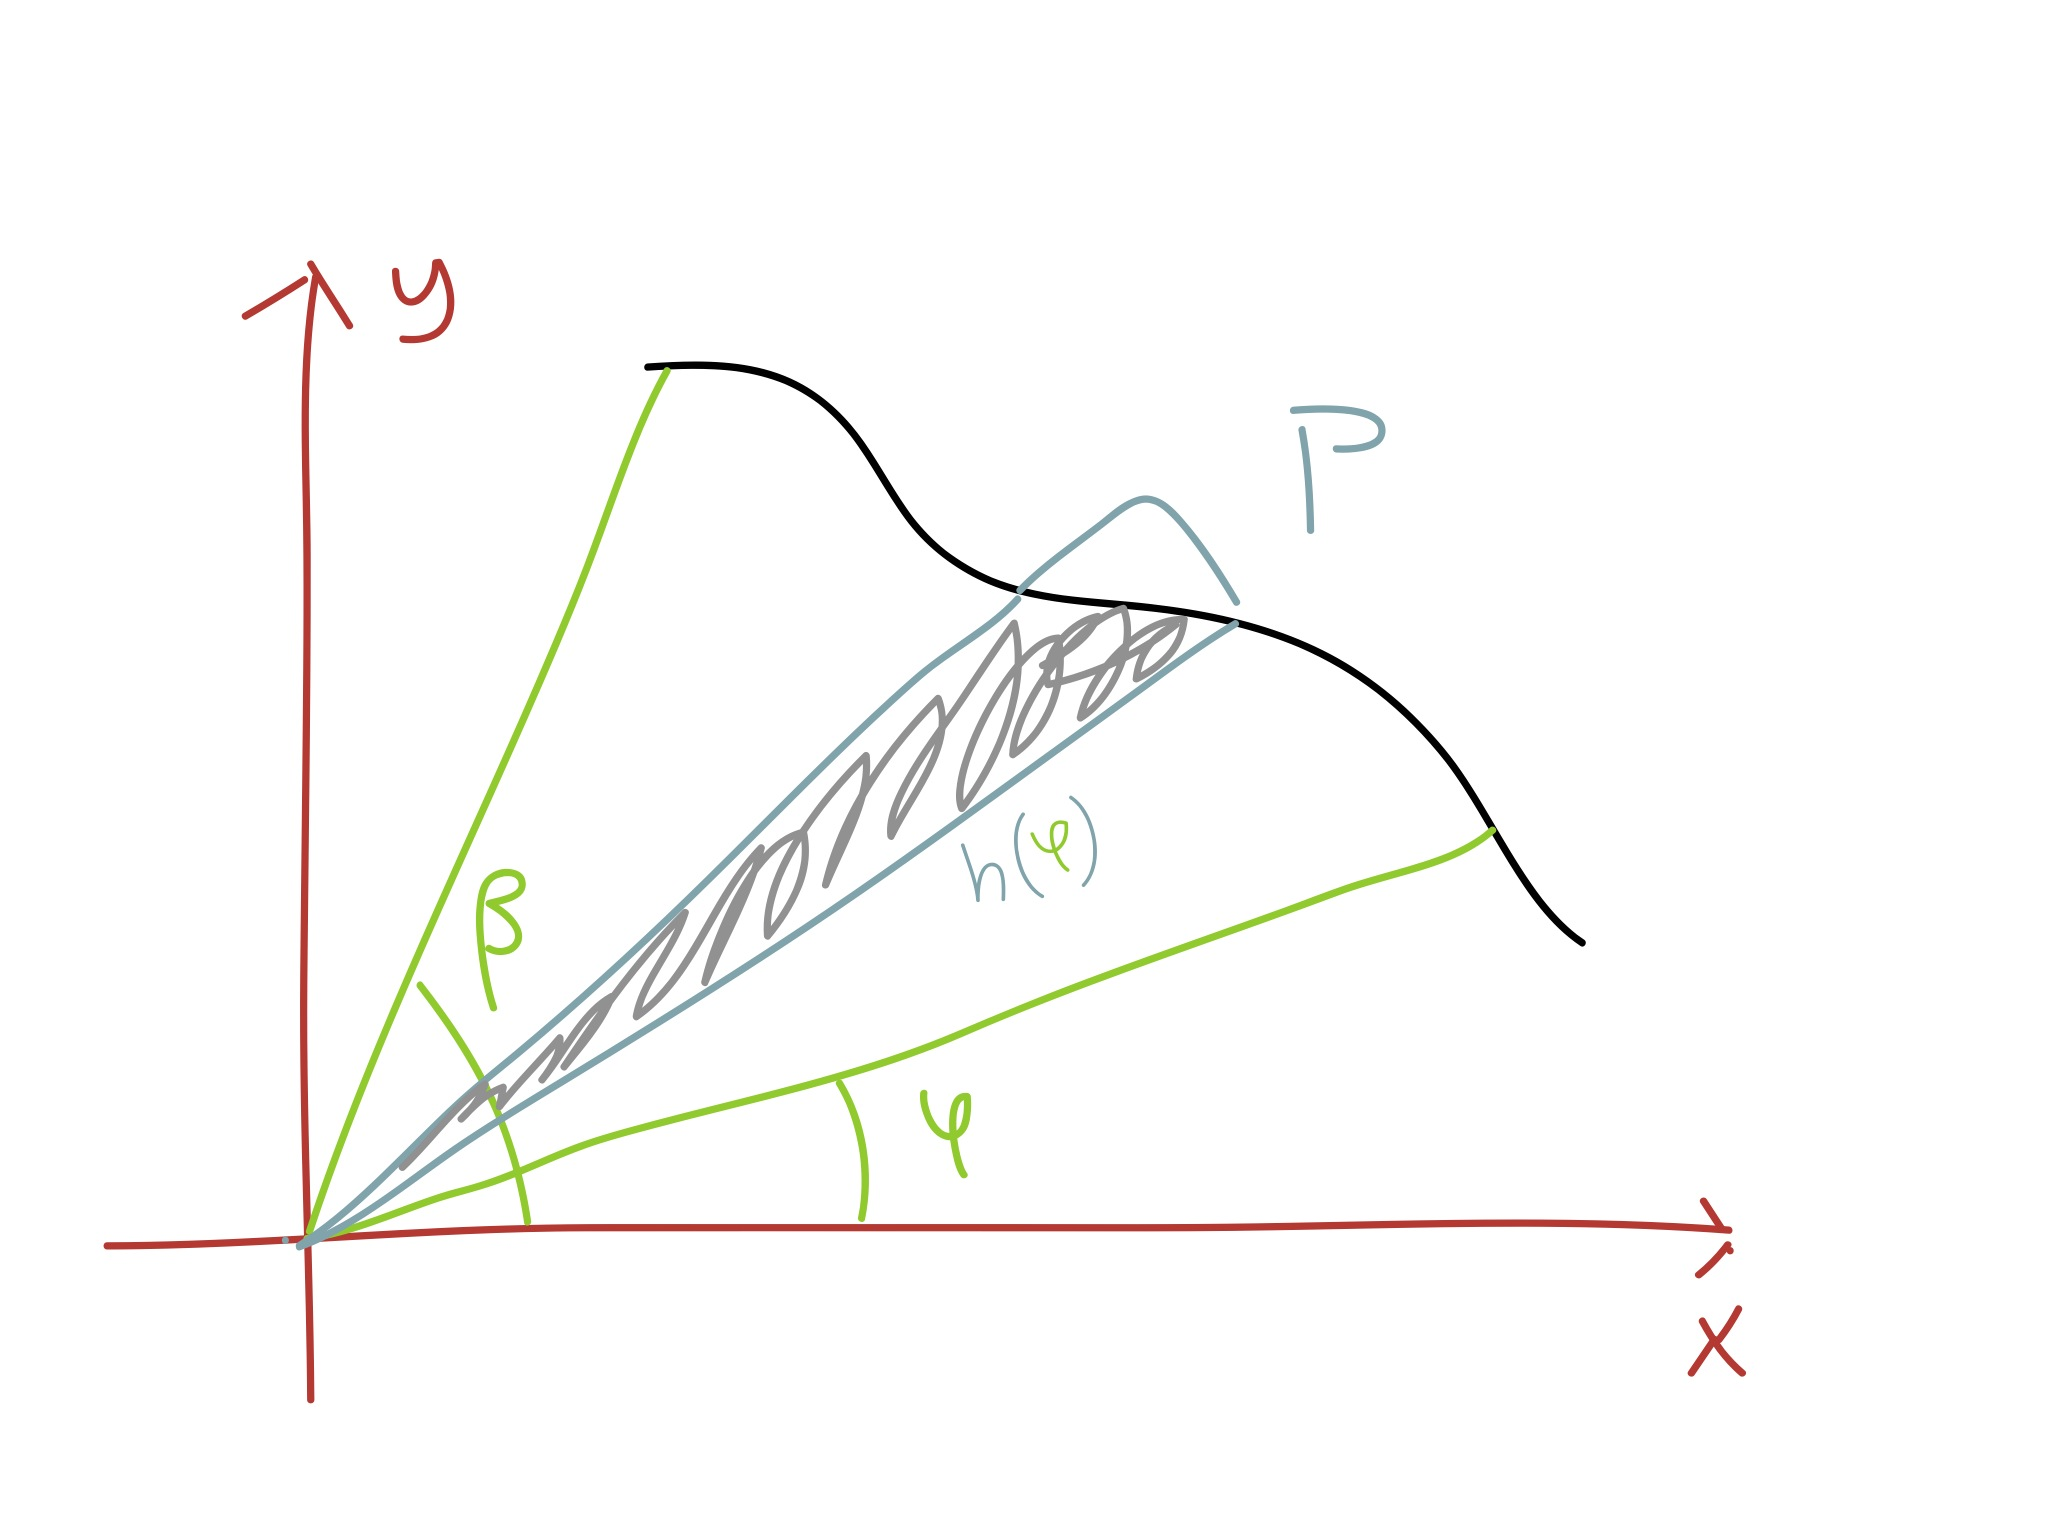
\includegraphics[scale=0.1]{img/img7.jpg}
% img 8
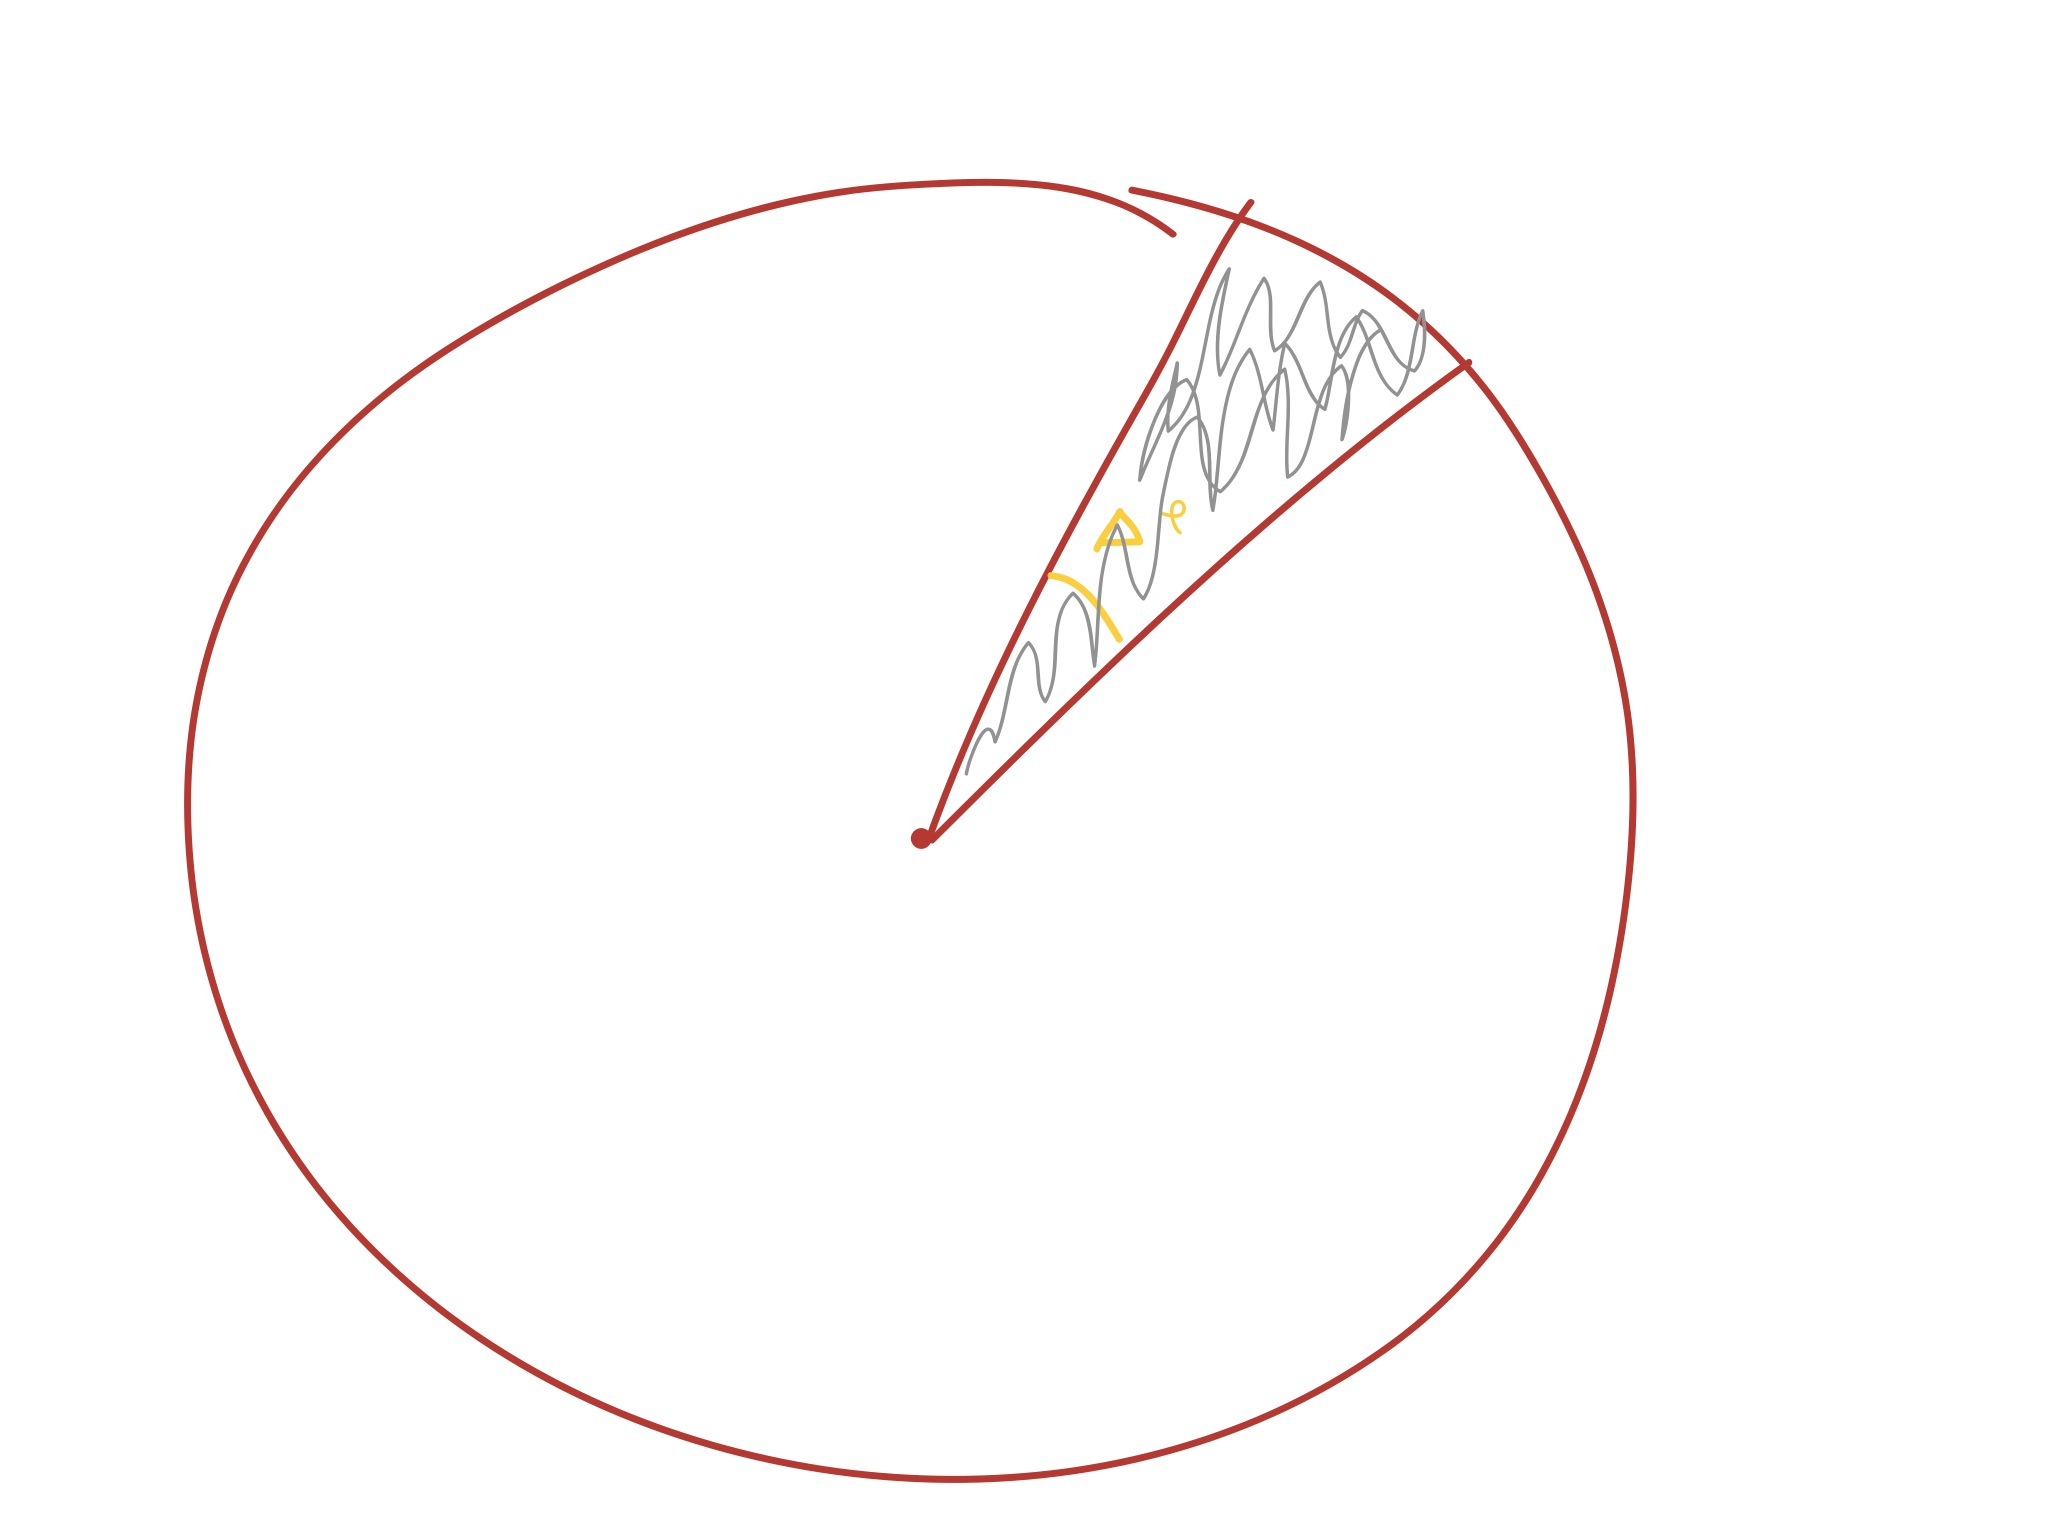
\includegraphics[scale=0.1]{img/img8.jpg}

$\Delta\phi$ är litet
$$ \Delta A = \f{\pi h^2(\phi)}{2\pi} * \Delta\phi $$

$$ A(D) = \sum \Delta A = \sum \f 12 h^2(\phi)\Delta\phi $$
$$ \Delta\phi \to 0 \im A(D) = \f 12 \int^\beta_\alpha{h^2(\phi)\ d\phi} $$

\subsection{Exempel 2}

En kurva ges i polära koordinater av $r=\phi, 0\le\phi\le 2\pi$
Bestäm arean av område som innesluts av kurvan.

% img 9
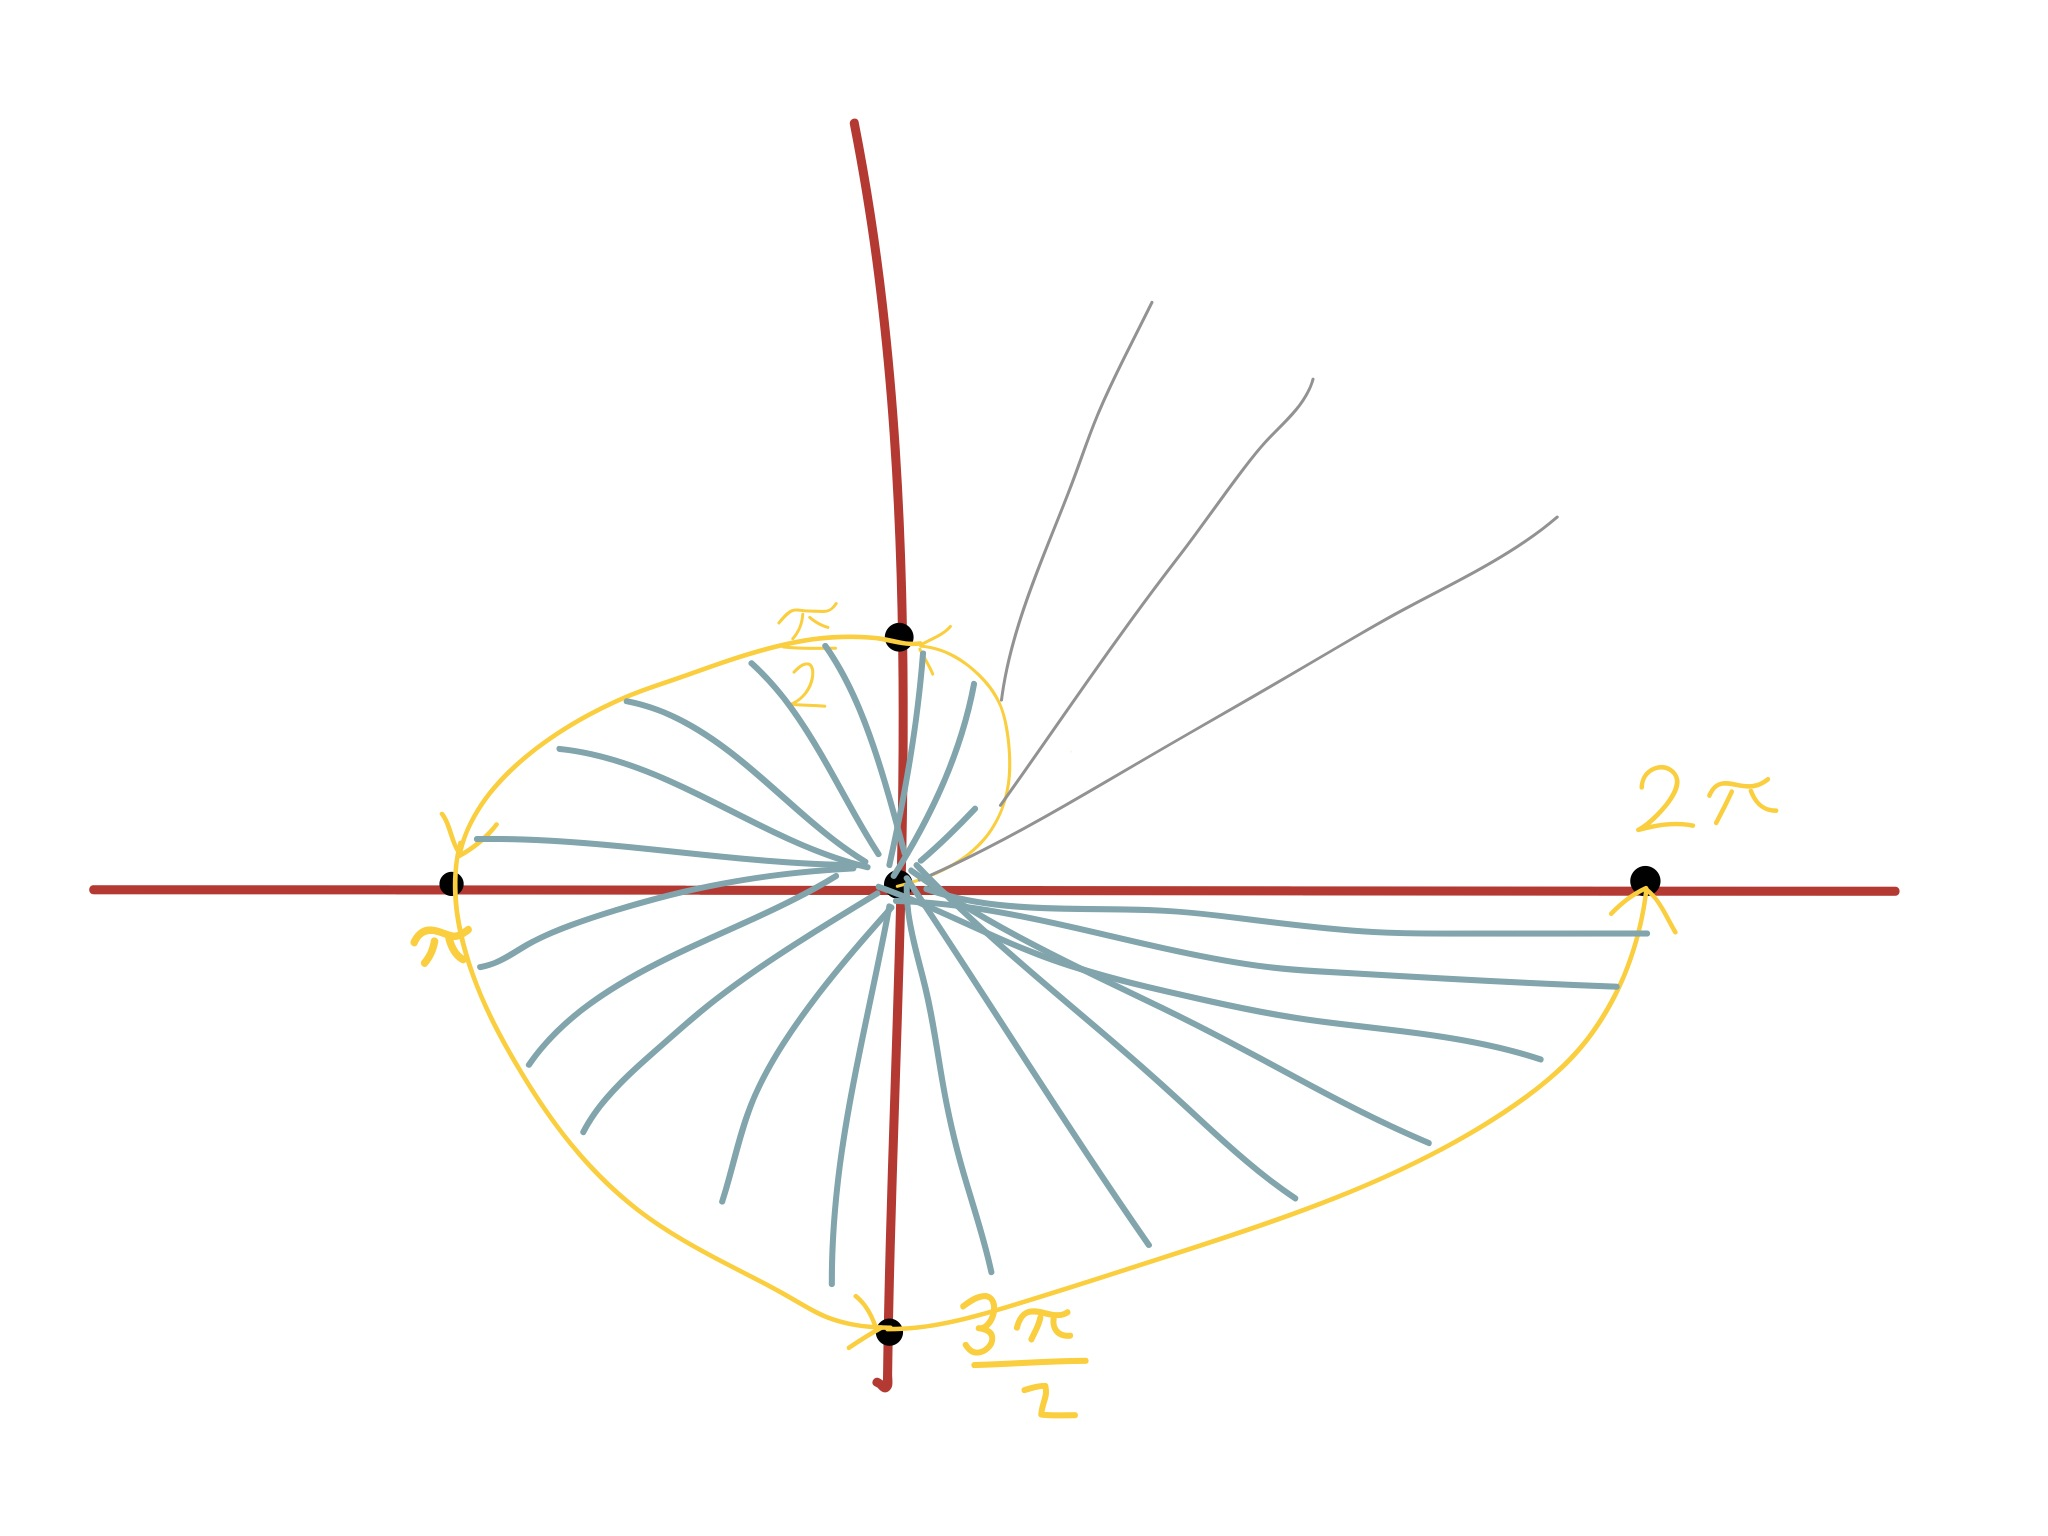
\includegraphics[scale=0.15]{img/img9.jpg}

$$
\begin{cases}
  \phi = 0\im r = 0\\
  \phi = \f\pi 2 \im r=\f\pi 2\\
  \phi = \pi\im r=\pi\\
  \phi = \f{3\pi}2\im r=\f{3\pi}2\\
\end{cases}
$$

$$ A(D) = \f 12 \int^{2\pi}_0{\phi^2\ d\phi} = \f 12\bra{\f 13 \phi^3}_{0}^{2\pi} = \f 43 \pi^3$$

\section{Kurvlängd}
\subsection{Kurvor på parameterform}

$$ x(t), y(t) $$ - kontinuerligt deriverbara

% img 10
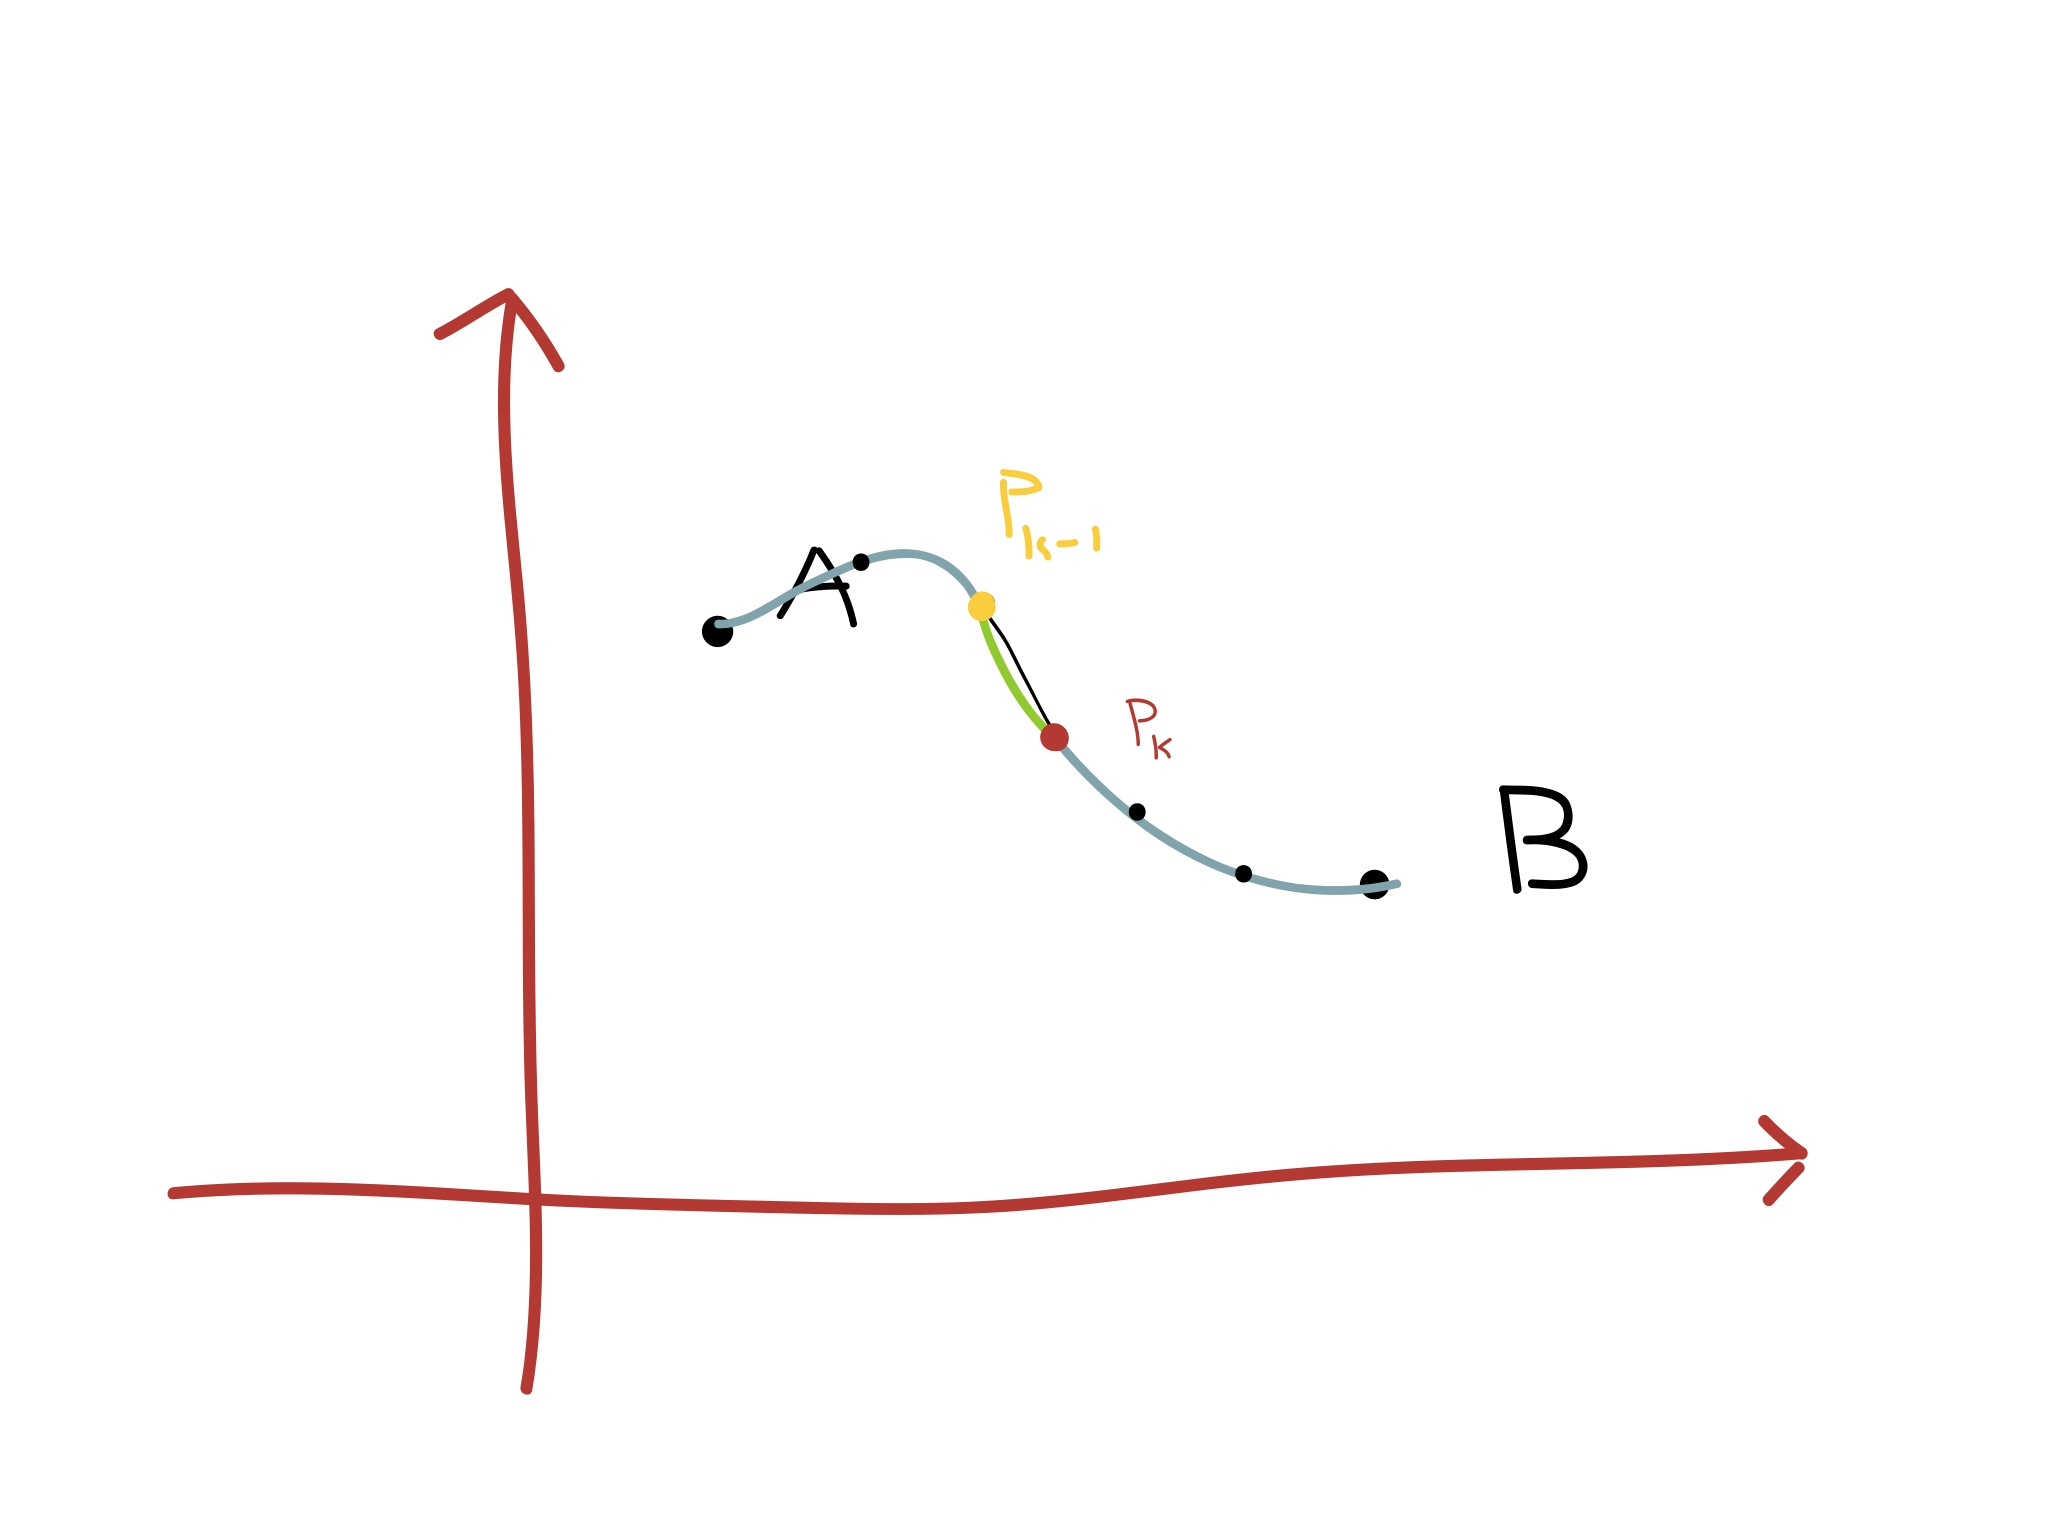
\includegraphics[scale=0.15]{img/img10.jpg}

$$ a\le t\le b $$
$$t \longmapsto (x(t), y(t)) $$

% img 11
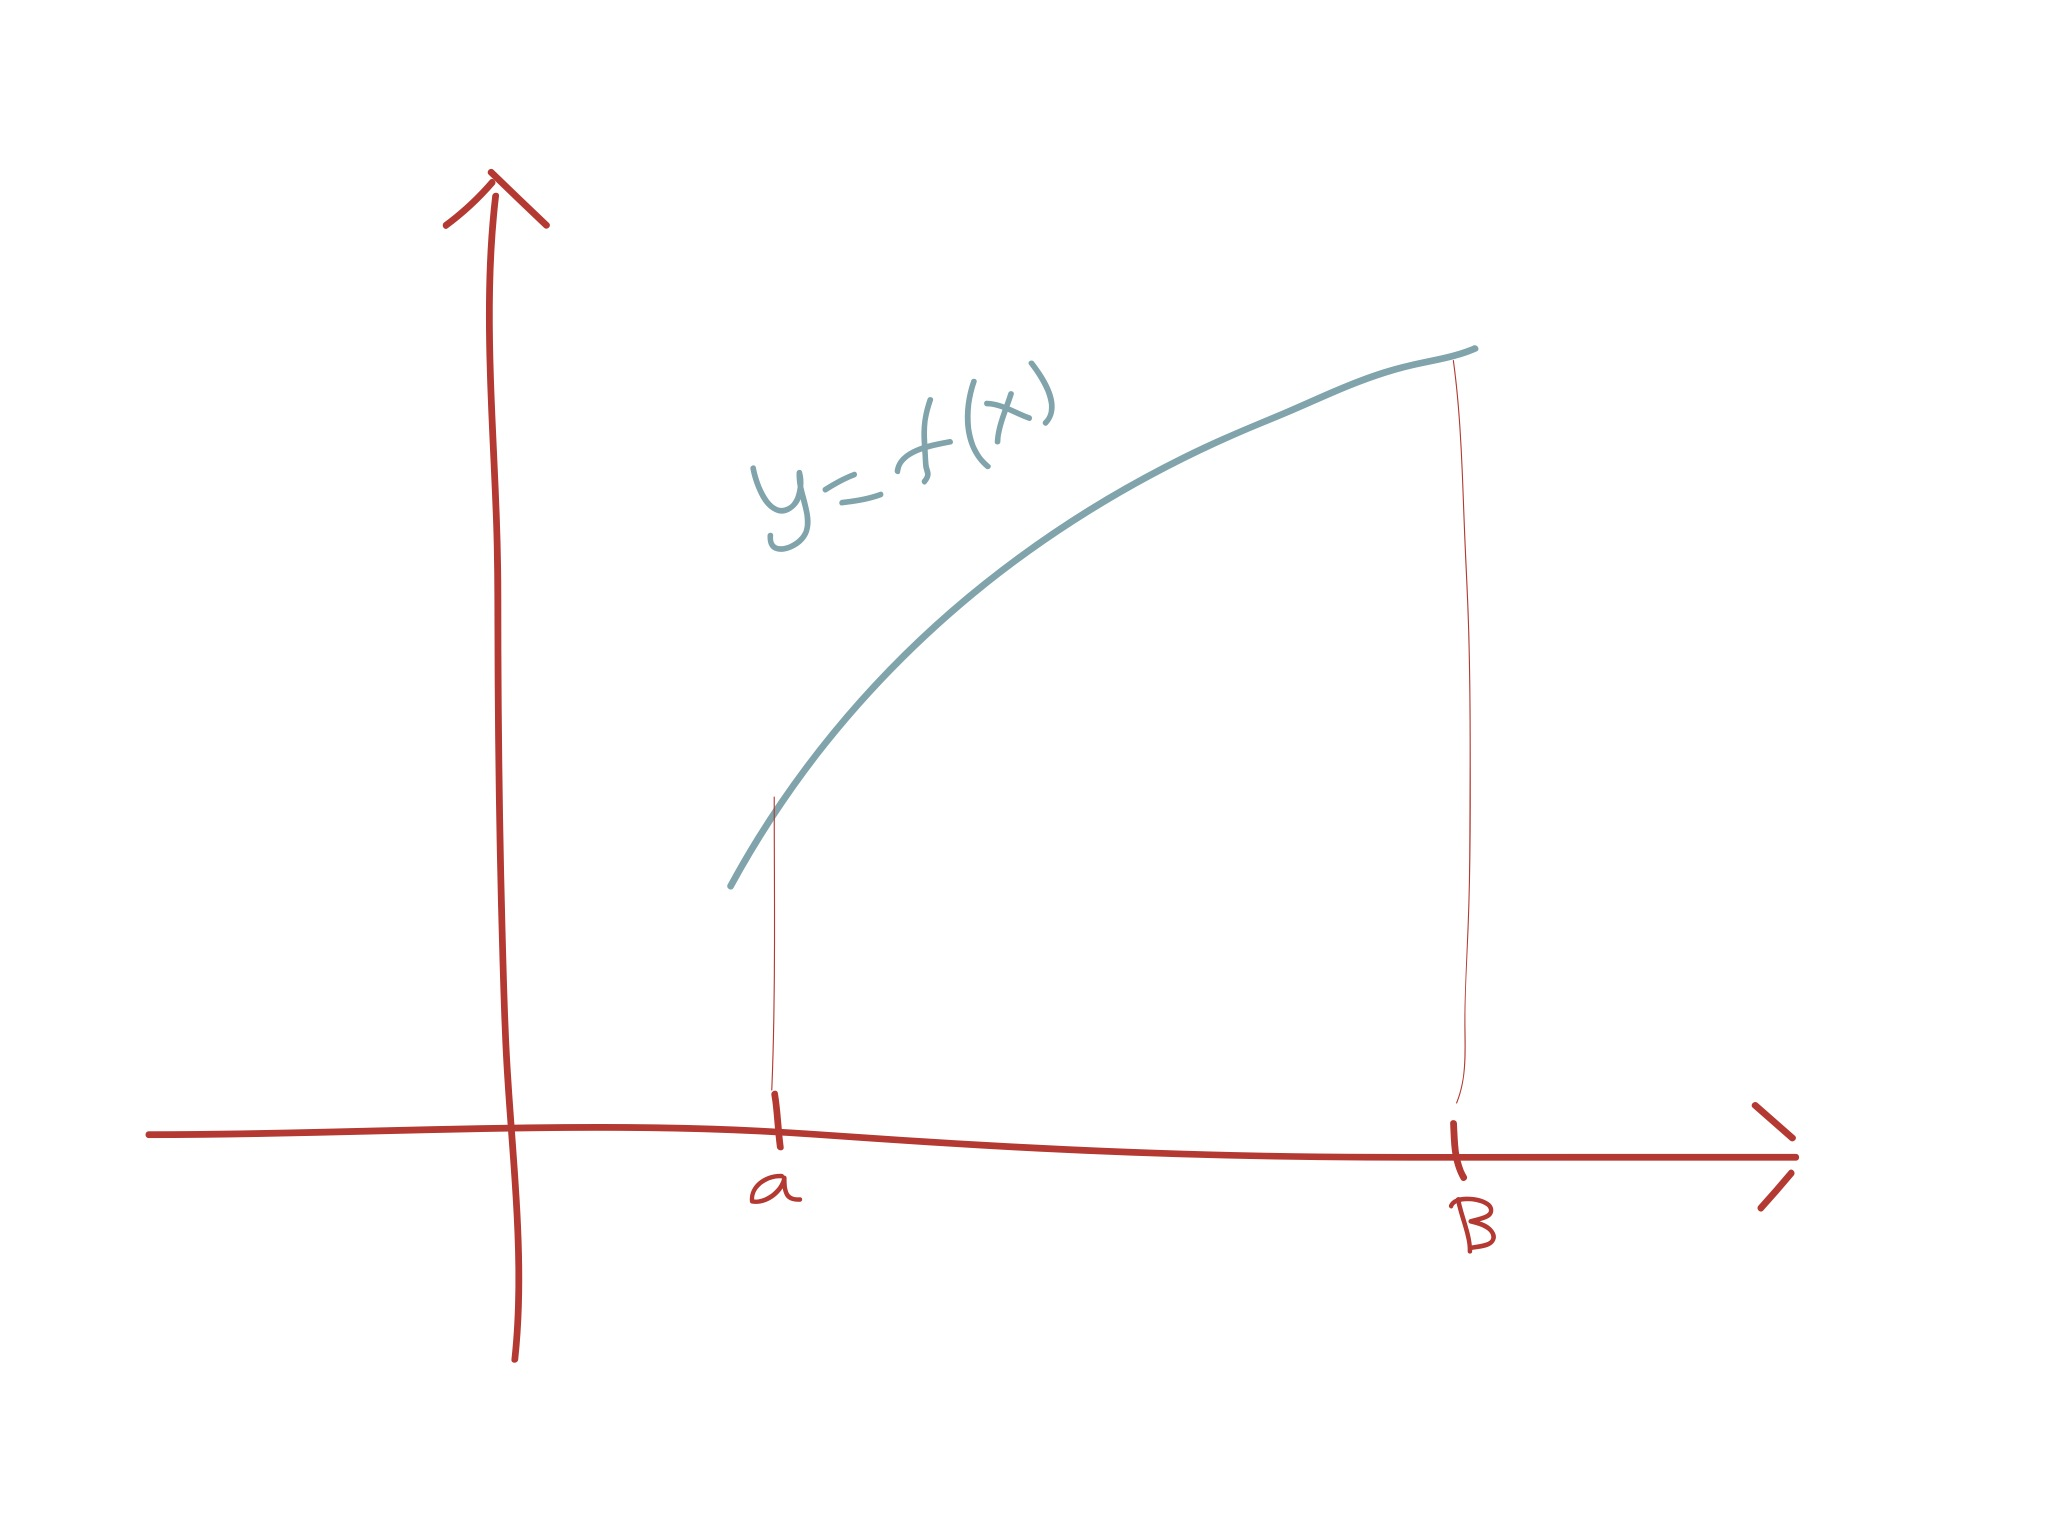
\includegraphics[scale=0.15]{img/img11.jpg}

$$ t=a\im(x(a), y(a)) = A $$
$$ t=b\im(x(b), y(b)) = B $$

$$ \Delta t_k = t_k - t_{k-1} $$

$$ \Delta s_k = \sqrt{(x(t_k)) - x(t_{k-1}))^2 + (y(t_k)) - y(t_{k-1}))^2 } =$$
$$\f{\sqrt{(\Delta x)^2 + (\Delta y)^2} * \Delta t_k}{\Delta t_k} =  $$
$$\sqrt{\f{(\Delta x)^2 + (\Delta y)^2}{\Delta t_k^2}}*\Delta t_k =  $$
$$\sqrt{\pa{\f{\Delta x}{\Delta t_k}}^2+\pa{\f{\Delta y}{\Delta t_k}}^2 } * \Delta t_k
\to \sqrt{x'^2 + y'^2}\ dt, \Delta t_k \to 0$$

$$ ds = \sqrt{x'^2 + y'^2}\ dt $$

$$ s = \int^b_a ds = \int^b_a{\sqrt{x'^2(t) + y'^2(t)}\ dt} $$

\subsection{Funktionskurvor}

% img 12
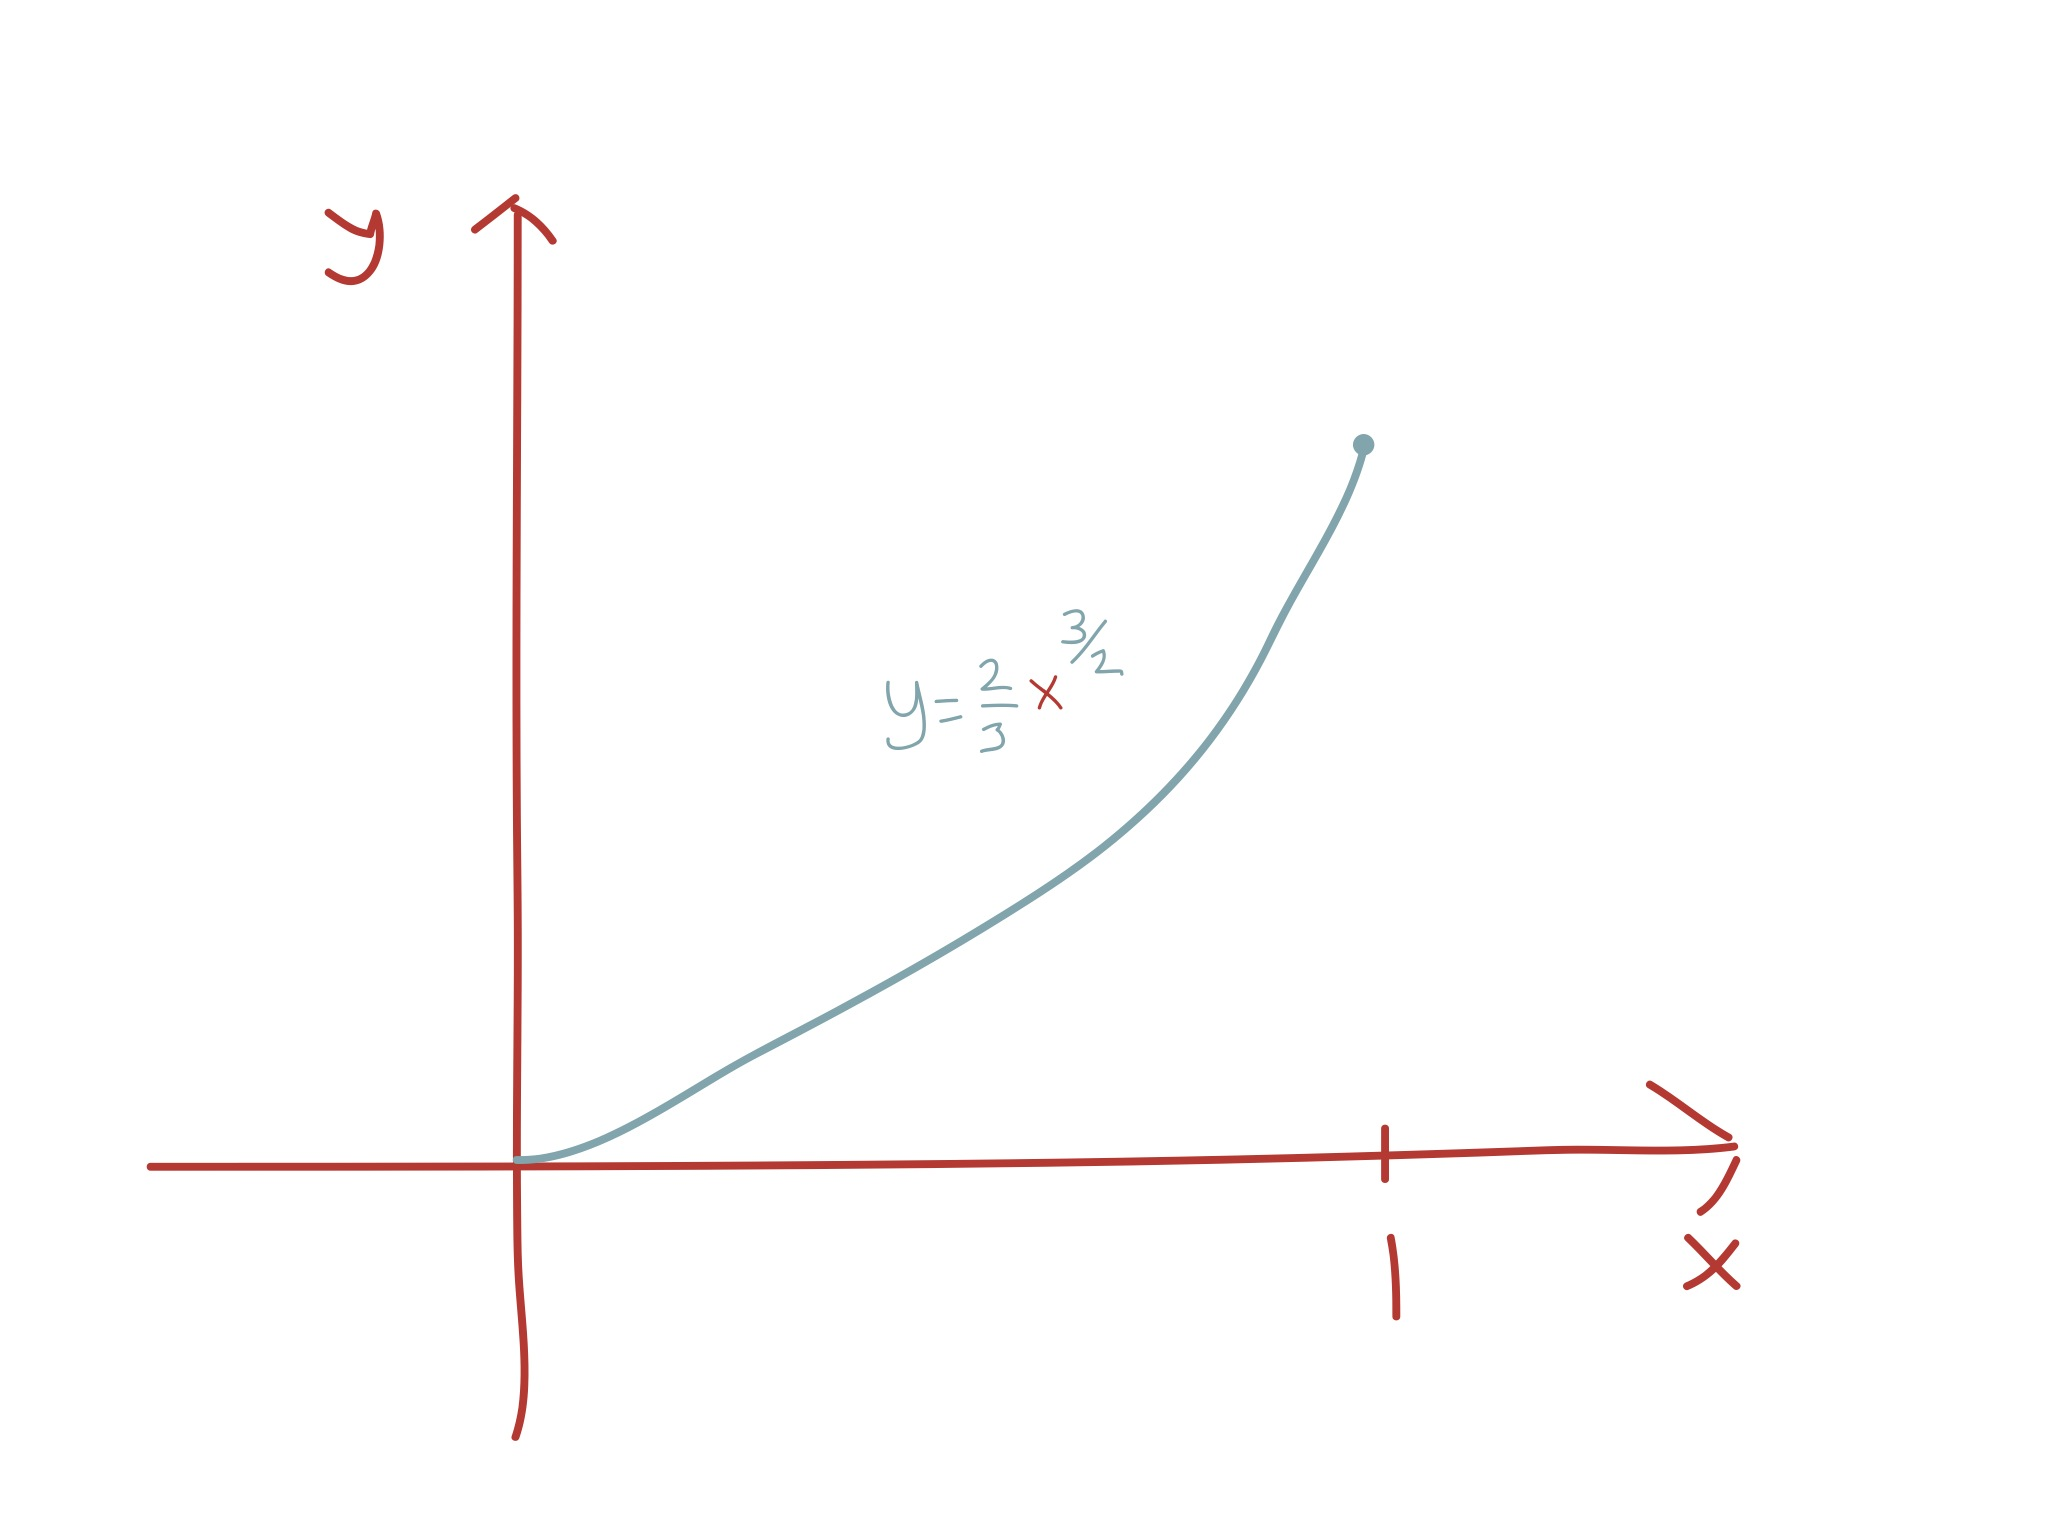
\includegraphics[scale=0.15]{img/img12.jpg}

$$ y = f(x), a\le x \le b $$

$$\begin{cases}
x=t, a\le t\le b\\
y=f(t)
\end{cases}$$

$$x'(t)=1 $$
$$y'(t)=f'(t)$$

$$ s=\int^b_a{\sqrt{1+f'^2(t)}\ dt} $$
$$ s=\int^b_a{\sqrt{1+f'^2(x)}\ dx} $$

\subsection{Exempel 3}

% img 13
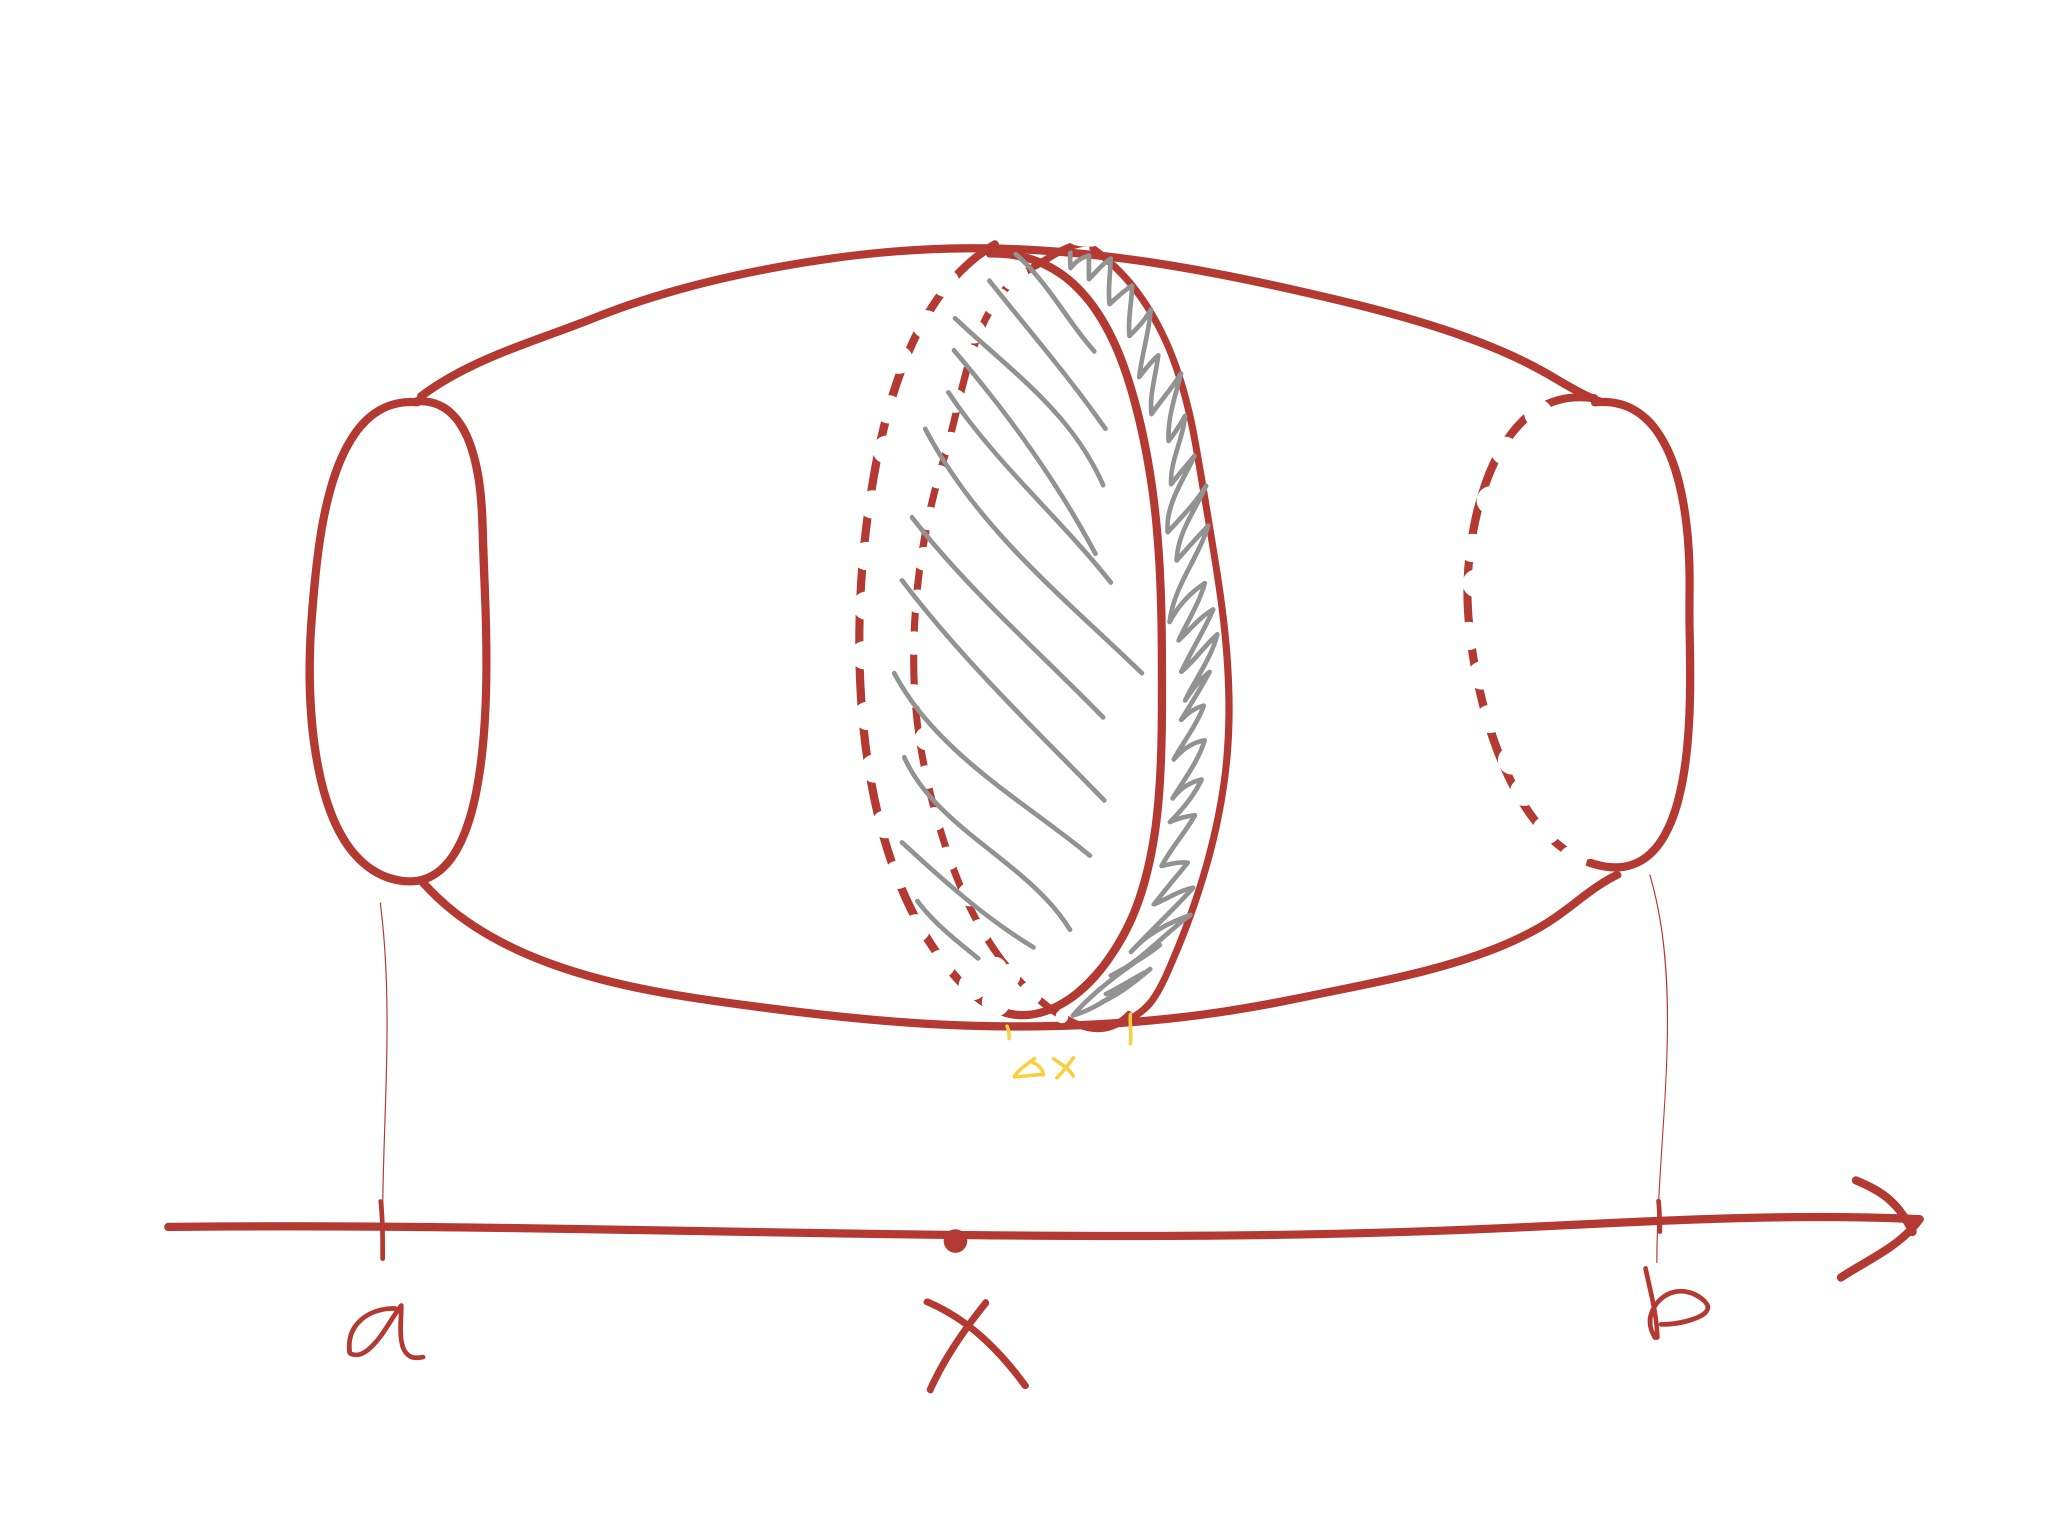
\includegraphics[scale=0.15]{img/img13.jpg}

Bestäm längden av $y=\f 23 x^{\f 32}, 0\le x\le 1$
$$f(x) = \f 23 x^{\f 32}$$
$$f'(x) = x^{\f 12} $$
$$ s=\int^1_0{1+x\ dx} = \bra{\f{{1+x}^{\f 32}}{\f 32}}^1_0 = \f 23 \pa{2\sqrt{2} - 1} $$

\section{Volym}

% img 14
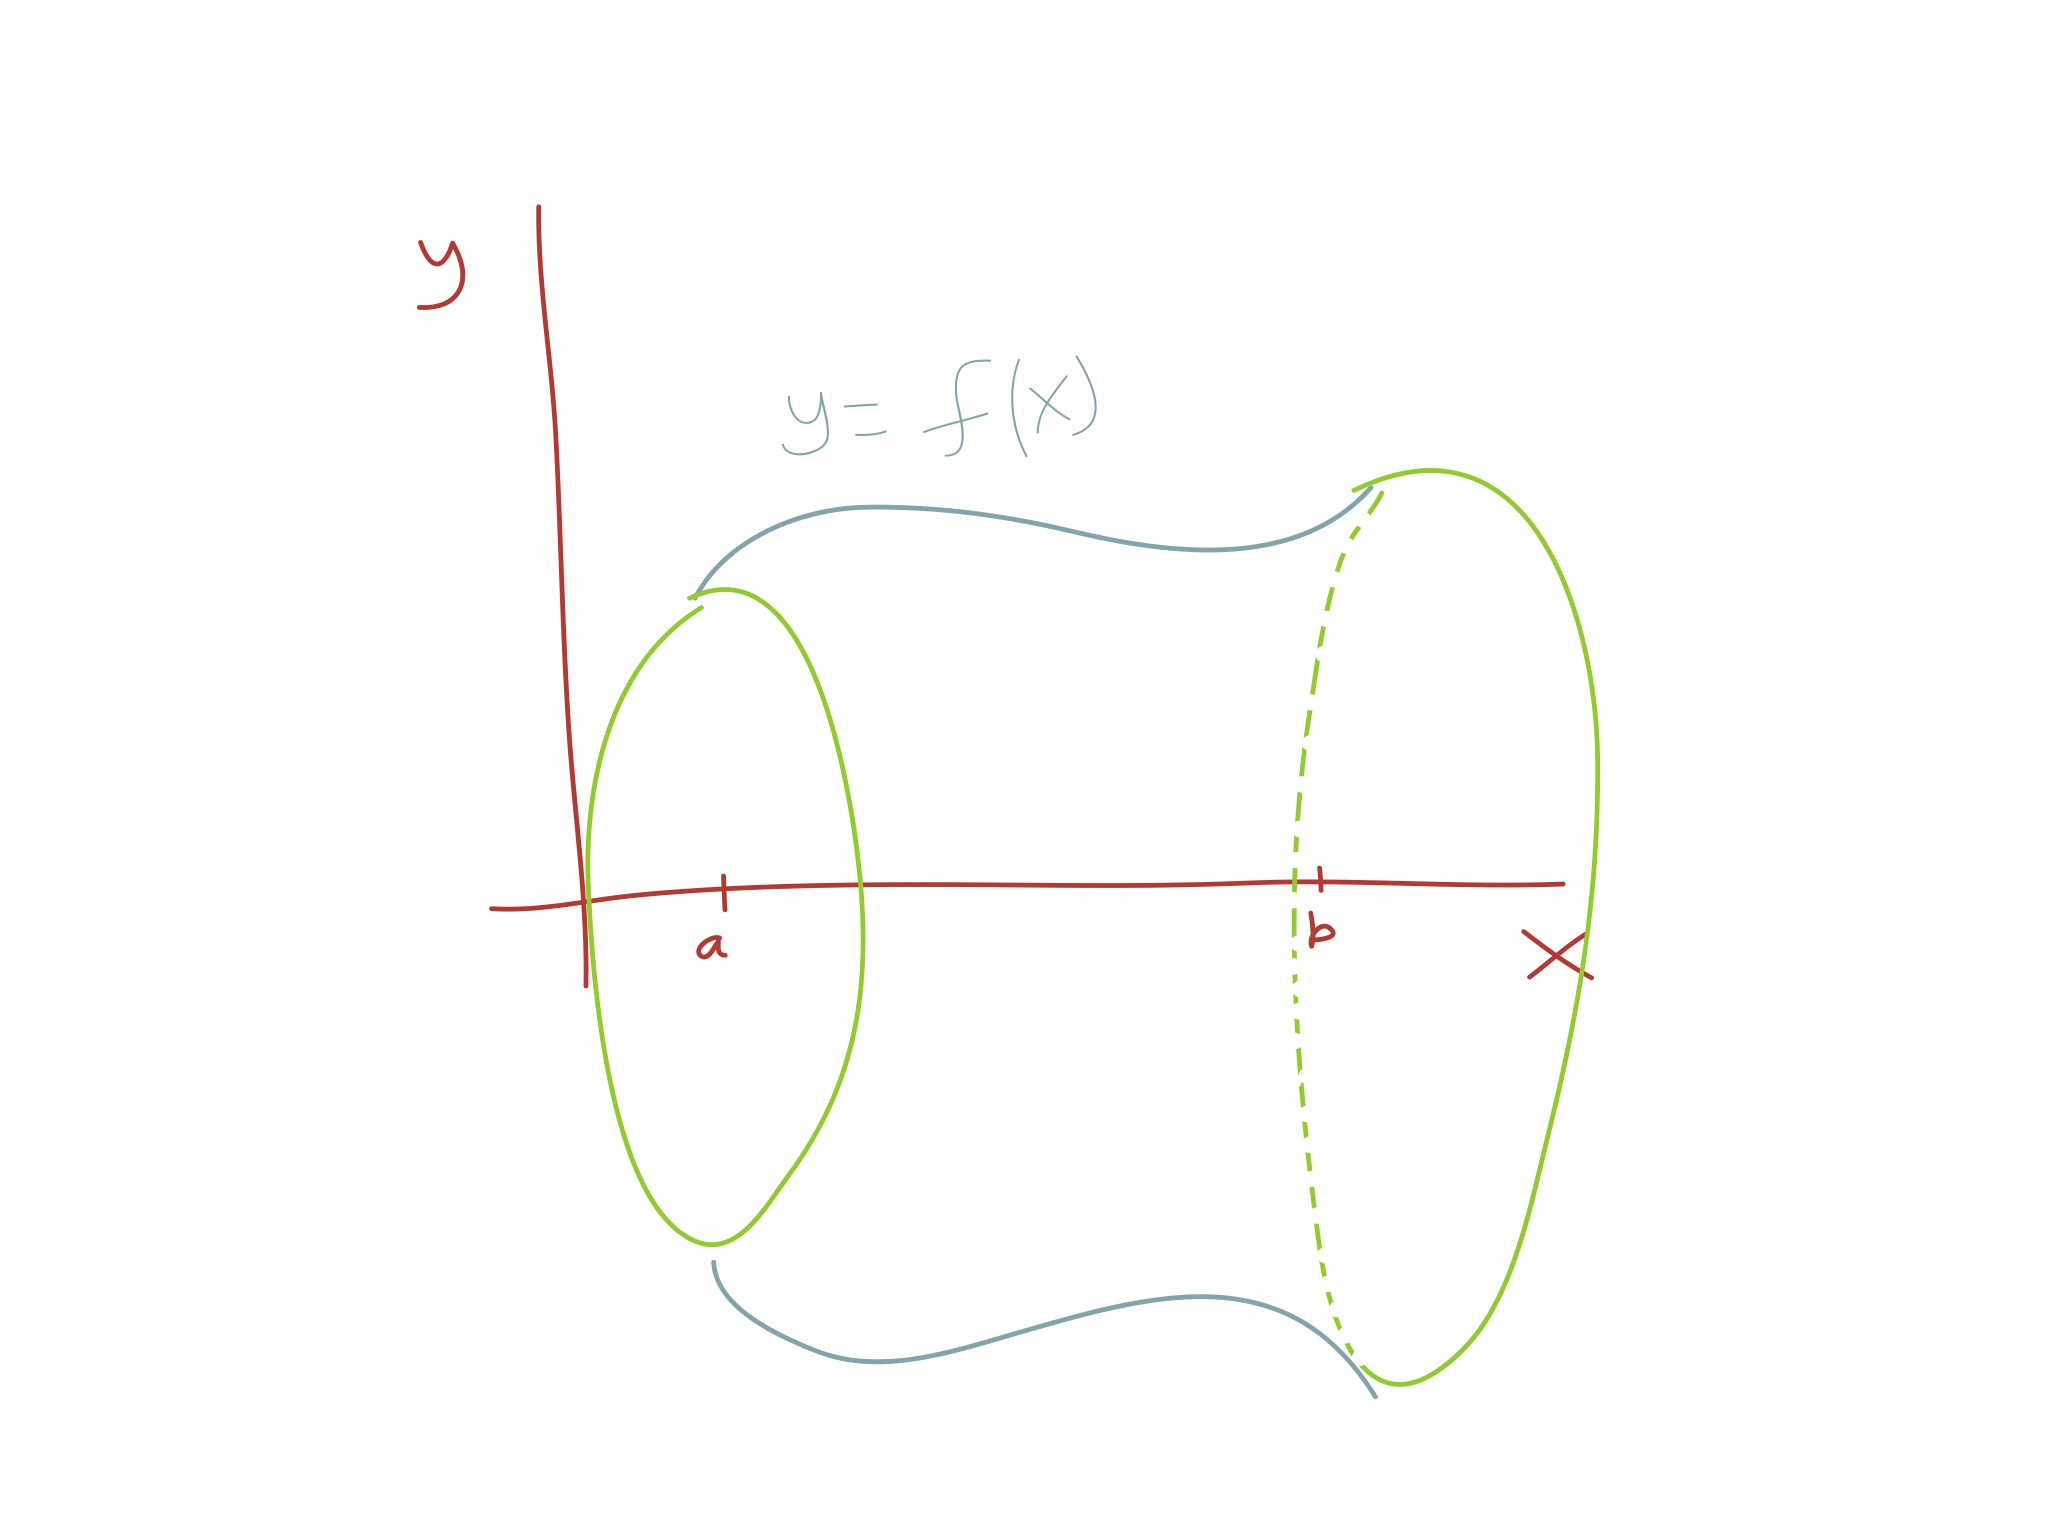
\includegraphics[scale=0.15]{img/img14.jpg}

$$ dV = A(x)\Delta x $$
$$ V=\int^b_a{A(x)\ dx} $$

\subsection{Rotationsvolym, skivformeln}

% img 15
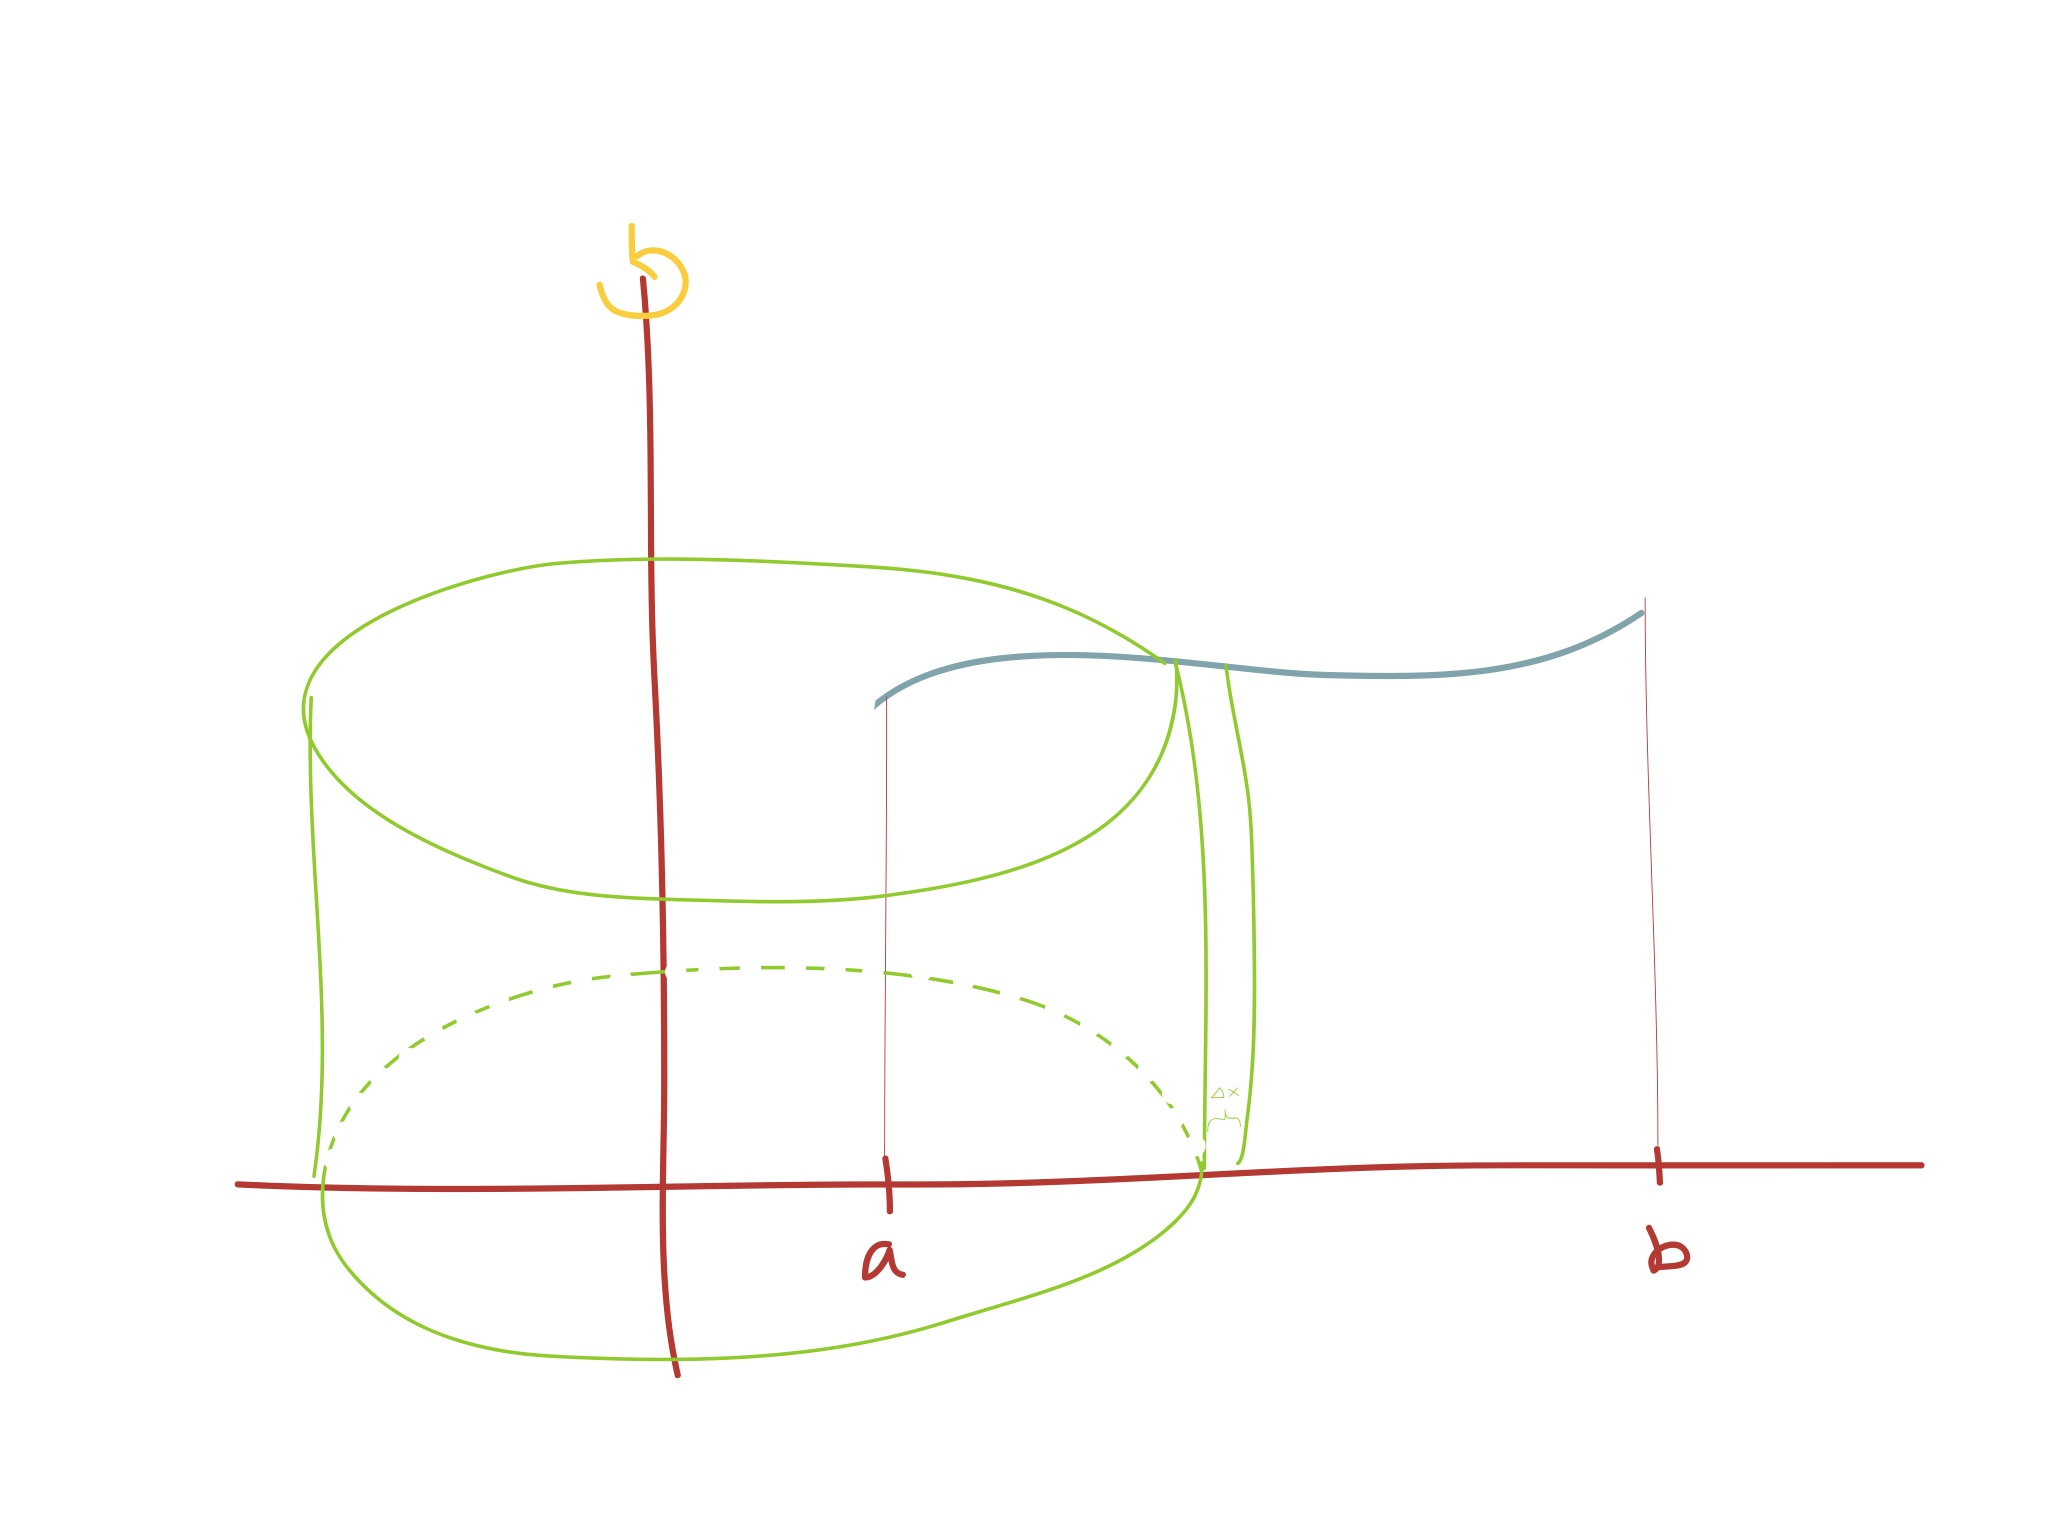
\includegraphics[scale=0.15]{img/img15.jpg}

$$ D=\{ (x,y) : a\le x\le b, 0\le y\le f(x) \} $$

$$A(x) = \pi f^2(x) $$

Skivformeln:
$$ V=\pi\int^b_a{f^2(x)\ dx} $$

\subsection{Rotationsvolym, rörformeln}

% img 16
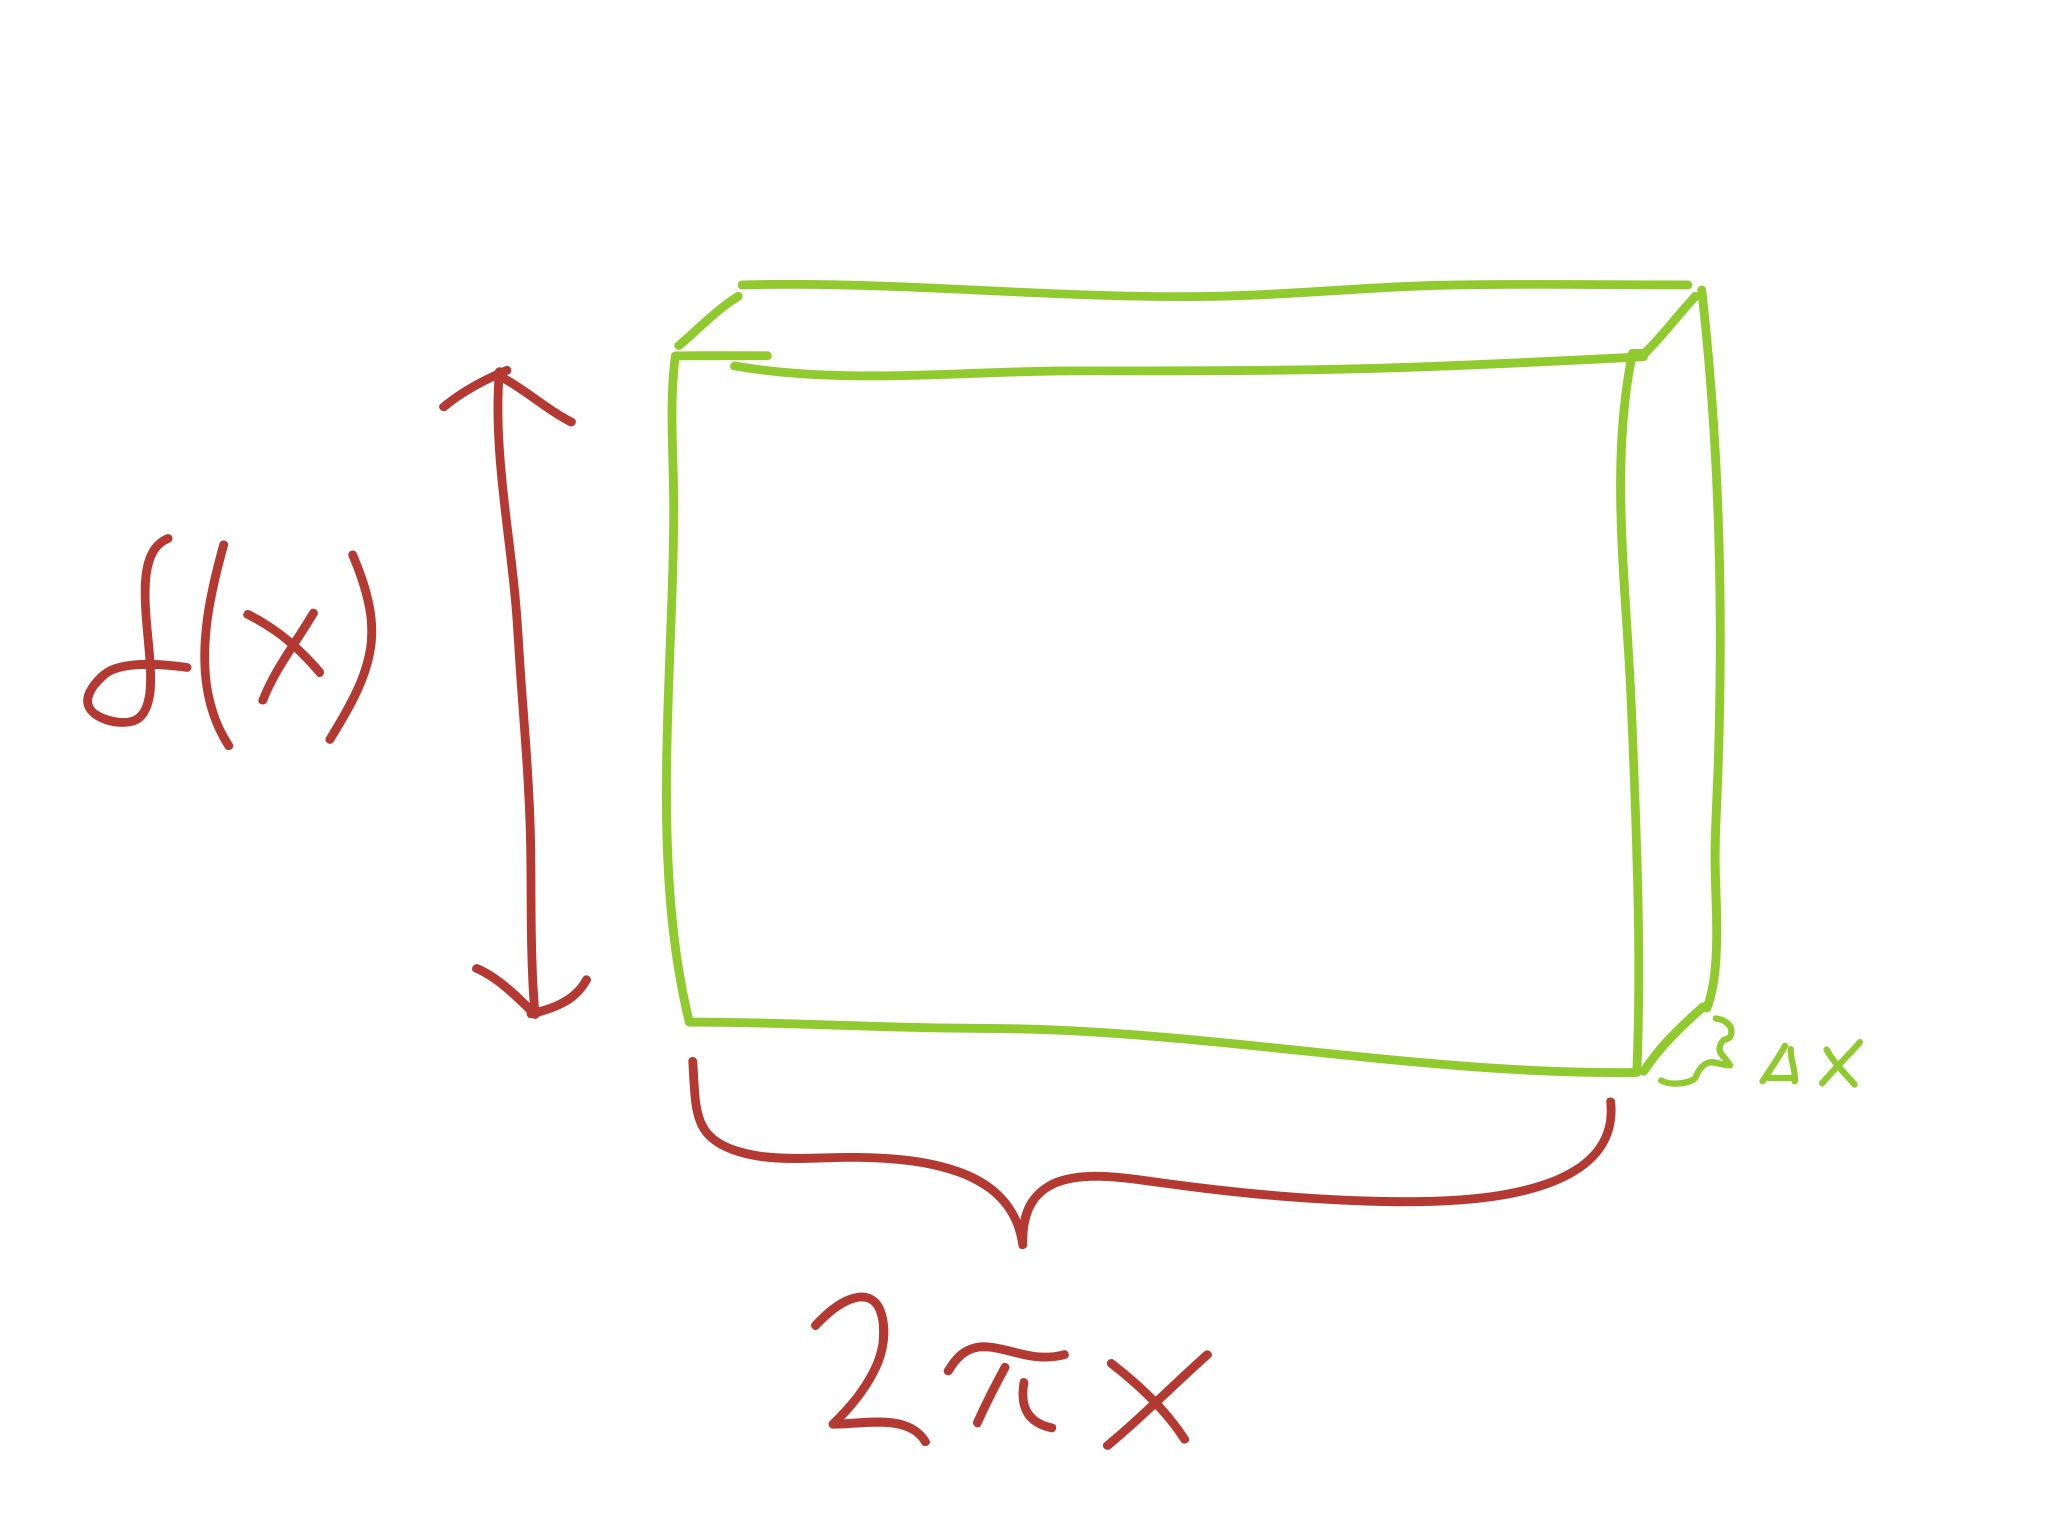
\includegraphics[scale=0.1]{img/img16.jpg}
% img 17
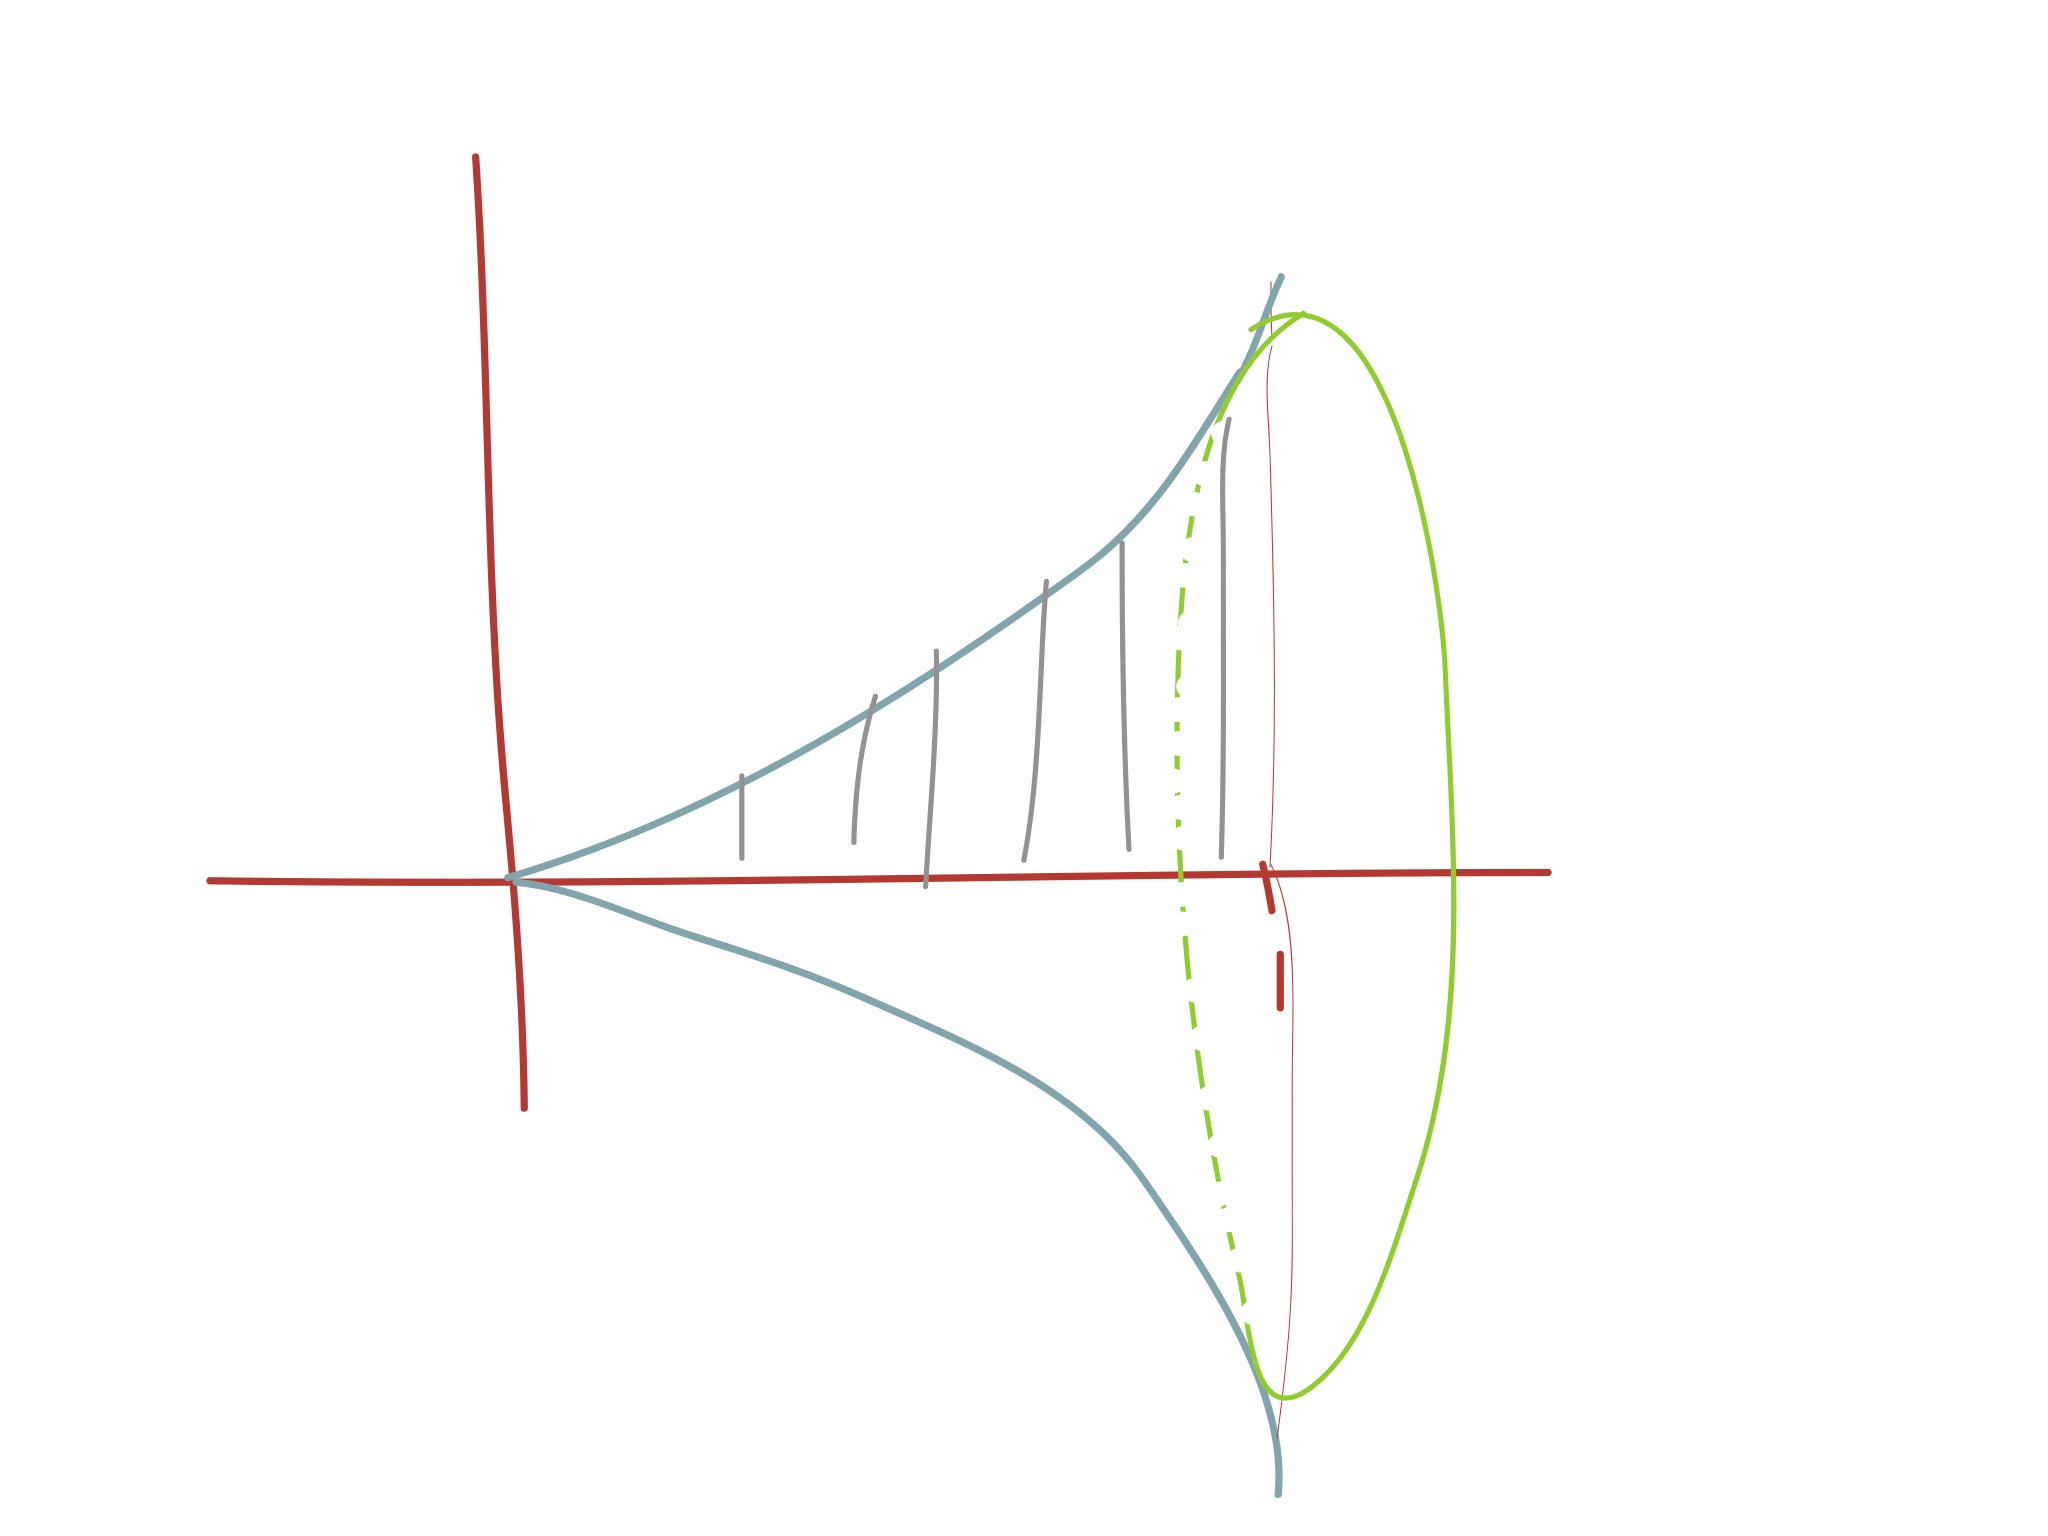
\includegraphics[scale=0.1]{img/img17.jpg}

$$ dV = 2\pi x f(x) \Delta x $$

Rörformeln:
$$ V = 2\pi\int^b_a{x f(x)\ dx} $$

\subsection{Exempel 4}

$$ D=\{ (x,y) : 0\le x\le 1, 0\le y\le x^2 \} $$
Roteras ett varv kring x-axeln.

$$ dV = \pi(x^2)^2\ dx$$
$$ V = \pi \int^1_0{x^4\ dx} = \bra{\pi\f{x^5}5}^1_0 = \f \pi 5 $$

Om $D$ roteras ett varv kring y-axeln.
$$ V=2\pi\int^1_0{x(x^2)\ dx}  = 2\pi\int^1_0{x^3\ dx} = 2\pi\bra{x^4\over 4}^1_0 = \f \pi 2$$


\end{document}
